\documentclass{beamer}

\mode<presentation> {


%\usetheme{default}
%\usetheme{AnnArbor}
%\usetheme{Antibes} 
%\usetheme{Bergen}
%\usetheme{Berkeley}
%\usetheme{Berlin}
%\usetheme{Boadilla}
%\usetheme{CambridgeUS}
%\usetheme{Copenhagen}
%\usetheme{Darmstadt}
%\usetheme{Dresden}
%\usetheme{Frankfurt}
%\usetheme{Goettingen}
%\usetheme{Hannover}
%\usetheme{Ilmenau}
%\usetheme{JuanLesPins}
%\usetheme{Luebeck}
\usetheme{Madrid}
%\usetheme{Malmoe}
%\usetheme{Marburg}
%\usetheme{Montpellier}
%\usetheme{PaloAlto}
%\usetheme{Pittsburgh}
%\usetheme{Rochester}
%\usetheme{Singapore}
%\usetheme{Szeged}
%\usetheme{Warsaw}
%\usecolortheme{albatross}
%\usecolortheme{beaver}
%\usecolortheme{beetle}
%\usecolortheme{crane}
%\usecolortheme{dolphin}
%\usecolortheme{dove}
%\usecolortheme{fly}
%\usecolortheme{lily}
%\usecolortheme{orchid}
%\usecolortheme{rose}
%\usecolortheme{seagull}
%\usecolortheme{seahorse}
%\usecolortheme{whale}
%\usecolortheme{wolverine}

%\setbeamertemplate{footline} % To remove the footer line in all slides uncomment this line
%\setbeamertemplate{footline}[page number] % To replace the footer line in all slides with a simple slide count uncomment this line

%\setbeamertemplate{navigation symbols}{} % To remove the navigation symbols from the bottom of all slides uncomment this line
}

\usepackage{graphicx} % Allows including images
\graphicspath{{/Users/justindoty/Documents/Research/Dissertation/Production_QR_Proxy/Code/}}
\usepackage{booktabs} % Allows the use of \toprule, \midrule and \bottomrule in tables
\usepackage{amsmath}
\usepackage{amssymb}
\usepackage{mathrsfs}
\usepackage{caption}
\usepackage{subcaption}
\usepackage{bbm} 
\usepackage{xcolor}
% \usepackage{natbib}
\usepackage[backend=biber, citestyle=apa, bibstyle=authoryear]{biblatex}
\addbibresource{references.bib}
%----------------------------------------------------------------------------------------
%	TITLE PAGE
%----------------------------------------------------------------------------------------

\title[Quantile Production Functions]{Heterogeneity in Firms:\\
A Proxy Variable Approach to Quantile Production Functions}

\author{Justin Doty and Suyong Song} % 
\institute[] % Your institution as it will appear on the bottom of every slide, may be shorthand to save space
{
\\  
\medskip % Your email address
}
\date{\today} % Date, can be changed to a custom date

\begin{document}

\begin{frame}
\titlepage % Print the title page as the first slide
\end{frame}

%----------------------------------------------------------------------------------------
%	PRESENTATION SLIDES
%----------------------------------------------------------------------------------------

%------------------------------------------------
\section{First Section} % Sections can be created in order to organize your presentation into discrete blocks, all sections and subsections are automatically printed in the table of contents as an overview of the talk
%------------------------------------------------

\subsection{Subsection Example} % A subsection can be created just before a set of slides with a common theme to further break down your presentation into chunks

\begin{frame}
\frametitle{Introduction}
\begin{itemize}
\item Identification issues: optimal input choices are functions of unobserved productivity leads to simultaneity bias
\item Popular control function approaches
\begin{itemize}
	\item \textcite{Olley1996}: Simultaneity and selection, investment policy proxy, application to telecommunications industry
	\item \textcite{Levinsohn2003}: Intermediate input proxy, application to Chilean manufacturing firms
	\item \textcite{Ackerberg2015}: Structural value-added production with intermediate input proxy, identification of labor elasticity
\end{itemize}
\item These approaches have focused on estimates of output elasticities on location of conditional firm-size distribution
\item There could be considerable heterogeneity not captured by average estimates
\end{itemize}
\end{frame}

%------------------------------------------------------------------------------------

\begin{frame}
\frametitle{Levinsohn and Petrin (2003)}
\begin{itemize}
	\item Brief review of LP approach	
	\item LP consider the following gross output production function
	\begin{equation}
	y_{it}=\beta_{0}+\beta_{k}k_{it}+\beta_{l}l_{it}+\beta_{m}m_{it}+\omega_{it}+\eta_{it}
	\end{equation}
	Where $\omega_{it}$ is productivity observed by the firm, but unobserved by the researcher (e.g, management quality, expected defect rates, etc.) and $\eta_{it}$ represents iid shocks to production after making input choices at time $t$
	With the following assumptions
	\medskip
	\begin{enumerate}
		\item Information Set: $\mathcal{I}_{it}$ includes current and past productivity shocks, but not future productivity. $\mathbb{E}[\eta_{it}|\mathcal{I}_{it}]=0$
		\item First Order Markov: Productivity shocks evolve according to the distribution $P(\omega_{it}|\omega_{it-1})$
		\item Capital Accumulation: $k_{it}=\kappa(k_{it-1}, i_{it-1})$
		\item Scalar Unobservability: $m_{it}=m_{t}(k_{it}, \omega_{it})$
		\item Strict Monotonicity: $m_{it}=m_{t}(k_{it}, \omega_{it})$ is strictly increasing in $\omega_{it}$
	\end{enumerate}
\end{itemize}
\end{frame}

%------------------------------------------------------------------------------------

\begin{frame}
\frametitle{Levinsohn and Petrin (2003)}
\begin{itemize}
	\item Given these assumptions intermediate input demand can be inverted $\omega_{it}=\omega_{t}(k_{it}, m_{it})$ and substituted into the production function
	\begin{equation}
		y_{it}=\beta_{0}+\beta_{k}k_{it}+\beta_{l}l_{it}+\omega_{t}(k_{it}, m_{it})+\eta_{it}=\beta_{l}l_{it}+\Phi(k_{it}, m_{it})+\eta_{it}
	\end{equation}
	where $\Phi(k_{it}, m_{it})=\beta_{0}+\beta_{k}k_{it}+\beta_{m}m_{it}+\omega_{t}(k_{it}, m_{it})$
	\item $\Phi(k_{it}, m_{it})$ can be estimated nonparametrically
	\item Labor coefficient and other variable coefficients are identified in the first stage
	\item First stage estimates are $\hat{\beta}_{l}$ and $\hat{\Phi}(k_{it}, m_{it})$ 
	\item Let $y^{*}=y-\hat{\beta}_{l}l_{it}$ denote the output net of labor contribution
\end{itemize}
\end{frame}

%------------------------------------------------------------------------------------

\begin{frame}
\frametitle{Levinsohn and Petrin (2003)}
\begin{itemize}
	\item Two moment conditions identify $\beta_{k}$ and $\beta_{m}$
	\item Capital does not respond to the innovation in productivity 
	\item Last period's input choice should not be correlated with the innovation in productivity this period
	\begin{equation}
	\mathbb{E}[(\eta_{it}+\xi_{it})Z_{it-1}]=\mathbb{E}[(y_{it}^{*}-\beta_{k}k_{it}-\beta_{m}m_{it}-\hat{\mathbb{E}}[\omega_{it}|\omega_{it-1}])Z_{it-1}]
	\end{equation}
	\item $\hat{\mathbb{E}}[\omega_{it}|\omega_{it-1}]$ can be estimated using the estimates of $\omega_{it}$ from first stage estimates evaluated at $(\beta_{k}, \beta_{m})$
	\item $Z_{it-1}$ includes $k_{it}$ and $m_{it-1}$ as well as additional instruments
	\item LP minimize GMM criterion function and bootstrap standard errors 
\end{itemize}
\end{frame}


%------------------------------------------------------------------------------------

\begin{frame}
\frametitle{Heterogeneous Coefficient Models}
\begin{itemize}
	\item \textcite{Kasahara2015} propose two methods to estimate a random coefficient production function and find evidence of unobserved heterogeneity beyond a Hicks-neutral technology term
	\item \textcite{balat} extend the control function approach to multi-dimensional coefficients with an application to international trade
	\item \textcite{Li2017} develop an identification strategy for heterogeneous elasticities using first order conditions for intermediate inputs
	\item \textcite{Gandhi2020} consider a nonparametric production function and a new identification argument in critique of proxy variables and explore heterogeneity in resulting TFP estimates
	\item \textcite{mert} uses a similar control variable approach to estimate output elasticities and markups. He finds that markup estimates using standard approaches are biased when both heterogeneity and labor-augmenting productivity are ignored
\end{itemize}
\end{frame}
%------------------------------------------------------------------------------------

\begin{frame}
\frametitle{Production Functions and Quantile Regression}
\begin{itemize}
	\item Allowing firm technology to vary over the conditional output distribution is also valid for estimating a production function with unobserved heterogeneity
	\item Alternative to splitting the sample on firm-size which may be inefficient and have arbitrary threshold selections which may lead to biased estimates
	\item Applications of quantile regression are however limited due to simultaneity bias
	\item Typical IV approaches such as \textcite{Chernozhukov2005} are also limited due problematic assumptions using input prices
	\item Possible to exploit the panel data structure and use fixed effects or correlated random effects such as \textcite{Koenker2004}, \textcite{Lamarche2010}, or \textcite{Canay2011}
	\item Incidental Parameters problem with quantile panel data
\end{itemize}
\end{frame}

%------------------------------------------------------------------------------------

\begin{frame}
\frametitle{Production Functions and Quantile Regression}
\begin{itemize}
	\item Quantile regression and production function estimation is not entirely new and has been used in the frontier literature
	\item Production frontier models assume firms are not always efficient, there is a frontier of maximal production in which they deviate from
	\item Stochastic frontier (SFA) models assume this frontier is stochastic (inefficiency + iid noise). These models are often characterized by strong distributional assumptions 
	\item Firms can vary in production technology for different levels of inefficiency making this model a strong candidate for quantile regression analysis \parencite{Bernini2004}, \parencite{Liu2008}
	\item Some difficulties of this approach is determining which quantiles correspond to the efficient frontier
	\item We believe we are the first to explore quantile regression in the standard production function literature, while also considering simultaneity bias
\end{itemize}
\end{frame}


%------------------------------------------------------------------------------------

\begin{frame}
\frametitle{A Random Coefficient Production Function}
We seek to extend the control function approach to a random coefficient value-production function defined as
\begin{equation} \label{qpf}
	y_{it}=\beta_{0}(\eta_{it})+\beta_{k}(\eta_{it})k_{it}+\beta_{l}(\eta_{it})l_{it}+\omega_{it}
\end{equation}
\begin{itemize}
	\item The interpretations of the variables in the above equation are the same as the LP model introduced earlier
	\item In this specification, the unobservable ranking variable, $\eta_{it}$ is responsible for heterogeneity in output conditional on firms using the same input combinations and latent productivity $\omega_{it}$
	\item If we had valid instruments, say $Z_{it}$ and the conditions of \textcite{Chernozhukov2005} are met, we could use quantile IV approaches using the identification condition
	\begin{equation}
	P(y_{it}\leq\beta_{0}(\tau)+\beta_{k}(\tau)k_{it}+\beta_{l}(\tau)l_{it}|k_{it}, l_{it}, Z_{it})=\tau
	\end{equation}
\end{itemize}
\end{frame}

%------------------------------------------------------------------------------------

\begin{frame}
\frametitle{Quantile Production Functions}
\begin{itemize}
	\item A special case of \eqref{qpf} is the location-scale model
	\small
	\begin{equation} \label{ls}
	y_{it}=\beta_{0}+\beta_{k}k_{it}+\beta_{l}l_{it}+\omega_{it}+(\mu_{0}+\mu_{k}k_{it}+\mu_{l}l_{it}+\mu_{\omega}\omega_{it})\eta_{it}
	\end{equation}
	\normalsize
	\item So the conditional quantiles of $y_{it}$ are given by
	\small
	\begin{equation}
	Q(y_{it}|k_{it}, l_{it}, \omega_{it})=\beta_{0}+\beta_{k}k_{it}+\beta_{l}l_{it}+\omega_{it}+(\mu_{0}+\mu_{k}k_{it}+\mu_{l}l_{it}+\mu_{\omega}\omega_{it})F^{-1}(\tau)
	\end{equation}
	\normalsize
	\item Equation \eqref{ls} is not new to the production function literature and is often used as a model for production risk \parencite{Just1978}
	\item They provide a set of postulates for which the above specification is empirically valid
	\item The quantile specification could be seen as an extension of the higher-order moment estimation of risk initiated by \textcite{Antle1983}
\end{itemize}
\end{frame}

%------------------------------------------------------------------------------------

\begin{frame}
\frametitle{Production Risk and Quantiles}
\begin{itemize}
	\item However, we do not seek to develop new theories of firm behavior under risk
	\item If one wanted to use production risk as an explanation of firm heterogeneity then it would be possible to use quantile utility maximization as the framework \parencite{Manski1988}, \parencite{Bhattacharya2009}, \parencite{ROSTEK2009}, \parencite{Chambers2007}, \parencite{Castro2017}
	\item It would then be possible to use the first order condition approach to estimate production function parameters using quantile regression techniques
	\item This approach is more difficult to synthesize in the proxy variable approach
	\item Which is why we consider production variation in $\eta_{it}$ to be an econometric misspecification issue rather than one that has any economic meaning
	\item Since most econometric tests would not be able to differentiate production risk from misspecification, we believe our interpretation to be equally as valid
\end{itemize}
\end{frame}

%---------------------------------------------------{}---------------------------------

\begin{frame}
\frametitle{Quantile Production Function: Assumptions}
\begin{itemize}
	\item We proceed with this interpretation and consider the production function specified in equation \eqref{qpf}
	\item We maintain several timing assumptions that are standard in the control function literature
\end{itemize}
\textbf{Assumption 1}
\begin{enumerate}
	\item Information Set: $\mathcal{I}_{it}$ includes current and past productivity shocks, but not future productivity. $\eta_{it}$ is independent of $\mathcal{I}_{it}$
	\item Firm's productivity follows an AR(1) process
	\begin{equation}
		\omega_{it}=g(\omega_{it-1}, \xi_{it})
	\end{equation}
	where $\xi_{it}$ are iid productivity innovations that is independent of $\mathcal{I}_{it-1}$
	\item Capital Accumulation: $k_{it}=\kappa(k_{it-1}, i_{it-1})$
	\item Scalar Unobservability: $m_{it}=m_{t}(k_{it}, \omega_{it})$
	\item Strict Monotonicity: $m_{it}=m_{t}(k_{it}, \omega_{it})$ is strictly increasing in $\omega_{it}$
\end{enumerate}
\end{frame}

%------------------------------------------------------------------------------------

\begin{frame}
\frametitle{Quantile Production Function: Estimation}
\begin{itemize}
	\item Given these assumptions we invert intermediate input demand $\omega_{it}=\omega_{t}(k_{it}, m_{it})$ and substitute into the production function \footnote{We subsume the constant $\beta_{0}(\eta_{it})$ into $\omega_{it}$}
	\begin{equation}
	y_{it}=\beta_{k}(\eta_{it})k_{it}+\beta_{l}(\eta_{it})l_{it}+\omega_{t}(k_{it}, m_{it})=\beta_{l}(\eta_{it})l_{it}+\Phi(k_{it}, m_{it}, \eta_{it})
	\end{equation}
	\item Using Assumption 1 we have:
	\begin{equation}
	P\big(y_{it}\leq \beta_{l}(\tau)l_{it}+\Phi(k_{it}, m_{it}; \tau)\big|\mathcal{I}_{it})=\tau
	\end{equation}
	\item If one uses a polynomial approximation to $\Phi_{\tau}(k_{t}, m_{t}; \tau)$, $\hat{\beta}_{l}(\tau)$ and $\hat{\Phi}(k_{t}, m_{t}; \tau)$ can be estimated using a polynomial quantile regression
	\item Substituting into the production
	\begin{equation}
	y_{it}=\beta_{k}(\eta_{it})k_{it}+\hat{\beta}_{l}(\tau)l_{it}+g(\hat{\Phi}(k_{it-1}, m_{it-1}; \tau)-\beta_{k}(\eta_{it})k_{it-1}, \xi_{it})
	\end{equation}
\end{itemize}
\end{frame}

%------------------------------------------------------------------------------------

\begin{frame}
\frametitle{Quantile Production Function: Estimation}
We can write a second stage restriction as
\begin{equation}
P\big(y_{it}\leq \beta_{k}(\tau)k_{it}+\hat{\beta}_{l}(\tau)l_{it}+g(\hat{\Phi}(k_{it-1}, m_{it-1}; \tau)-\beta_{k}(\tau)k_{it-1}; \tau)|\mathcal{I}_{it-1}\big)=\tau
\end{equation}
This can be represented by conditional moment restrictions
	\begin{equation}
	\begin{split}
	\mathbb{E}[\mathbbm{1}\{y_{it}&-\beta_{k}(\tau)k_{it}-\hat{\beta}_{l}(\tau)l_{it}\\
	&+g(\hat{\Phi}(k_{it-1}, m_{it-1}; \tau)-\beta_{k}(\tau)k_{it-1}; \tau)\leq 0\}-\tau|\mathcal{I}_{it-1}]=0
	\end{split}
	\end{equation}
	where $\mathbbm{1}\{\cdot\}$ is the indicator function
To estimate the production function parameters we use the unconditional moments
	\begin{equation}
	\begin{split}
	\mathbb{E}[Z_{it-1}(\mathbbm{1}\{y_{it}&-\beta_{k}(\tau)k_{it}-\hat{\beta}_{l}(\tau)l_{it}\\
	&+g(\hat{\Phi}(k_{it-1}, m_{it-1}; \tau)-\beta_{k}(\tau)k_{it-1}; \tau)\leq 0\}-\tau)]=0
	\end{split}
	\end{equation}
	where $Z_{it-1}$ includes the instruments used in the firm's information set at time $t-1$
	
\end{frame}
%------------------------------------------------------------------------------------

\begin{frame}
\frametitle{Smoothed GMM for Quantile Models}
\begin{itemize}
	\item The indicator function makes estimation of the production function parameters intractable
	\item We smooth the indicator function and rely on estimation procedure of \textcite{Kaplan2016}
	\item \textcite{qgmm} develop theory for feasible estimators of parameters in general conditional quantile restrictions that include non-linear IVQR
	\item This approach is computationally attractive compared to approaches such as the MCMC approach proposed by \textcite{Chernozhukov2003}
	\item To fix notation let
	\begin{itemize}
		\item $Z_{it-1}$ the set of instruments discussed earlier
		\item $x_{it}$ the set of exogenous and endogenous covariates
		\item $\Lambda(\cdot)$ denote the residual function that defines the conditional quantile restriction that is known up to $\beta_{k}(\tau)$
	\end{itemize}
	
\end{itemize}
\end{frame}
%------------------------------------------------------------------------------------

\begin{frame}
\frametitle{Smoothed GMM for Quantile Models}
\begin{itemize}
	\item The sample analog of (12) can be written as:
	\begin{equation}
    \hat{M}_{n}(\beta, \tau)=\frac{1}{NT}\sum_{i=1}^{N}\sum_{t=1}^{T}Z_{it}\Bigg[\tilde{I}\Bigg(\frac{\Lambda(y_{it}, x_{it}, \beta(\tau))}{h_{n}}\Bigg)-\tau\Bigg],
	\end{equation}
	where $h_{n}$ is a bandwidth (sequence) and $\tilde{I}(\cdot)$ is a smoothed version of the indicator function $\mathbbm{1}\{\cdot \leq 0\}$ used by \textcite{Horowitz1998}, \textcite{Whang2006}, and \textcite{Kaplan2016}:
	\begin{equation}
	    \tilde{I}(u)=\mathbbm{1}\{-1\leq u \leq 1\}\big[0.5+\frac{105}{64}\big(u-\frac{5}{3}u^{3}+\frac{7}{5}u^{5}- \frac{3}{7}u^{7}\big)\big]+\mathbbm{1}\{u>1\}.
	\end{equation}
	The smoothed GMM estimator minimizes a weighted quadratic norm of the smoothed sample moment vector
	\begin{equation}
		\hat{\beta}_{GMM}=\underset{\beta}{\operatorname{argmin}}\hat{M}_{n}(\beta, \tau)^{\top}\hat{W}\hat{M}_{n}(\beta, \tau).
		\end{equation}
\end{itemize}
\end{frame}

%------------------------------------------------------------------------------------

\begin{frame}
\frametitle{Smoothed GMM for Quantile Models}
\begin{itemize}
	\item The optimal weighting matrix is the estimator of the inverse long-run variance of the sample moment $\hat{W}^{*}=\bar{\Omega}^{-1}\overset{p}{\to}\Omega^{-1}$
	\item In simulation and in application we use an estimate of the long-run variance using a truncated kernel with bandwidth choice of \textcite{Andrews1991}. We find this helps with scaling.
	\item The asymptotic results for this estimator cannot be applied here due to the semi-parametric nature of the two-step procedure
	\item The asymptotic results of \textcite{Ai2007} could be applied here. 
	\item This gives us extra conditions to show what rate gives an asymptotically negligible bandwidth. The smoothed sample moments are differentiable so we can take a Taylor expansion around $\beta(\tau)$. We leave this for future research agenda
	\item Therefore we use the bootstrap in our empirical application
	\item Optimal choice of bandwidth is an ongoing research topic for these types of estimators. We use very small (h=1e-6) throughout 
\end{itemize}
\end{frame}

%------------------------------------------------------------------------------------

\begin{frame}
\frametitle{Quantile Production Function: Simulation}
\begin{itemize}
	\item Simulations follow a location-scale version of LP and ACF using ACF's original set of DGPs 
	\item Parameters are chosen to match a couple of key moments in the Chilean data used by LP
	\item Productivity follows a first order AR(1) process with persistence $\rho=0.7$
	\item Firms make optimal choices of investment in the capital stock to maximize the expected discounted value of future profits
	\item Convex capital adjustment costs
	\item Labor input $l_{it}$ is chosen either at $t$ or $t-b$
	\item Possible optimization error in labor input decision
\end{itemize}
\end{frame}

%------------------------------------------------------------------------------------

\begin{frame}
\frametitle{Monte Carlo Simulation}
\begin{itemize}
	\item Production function is assumed Leontief in materials, the location-scale specification is
	\begin{equation}
		y_{t}=\beta_{k}k_{it}+\beta_{l}l_{it}+\omega_{it}+(0.7k_{it}+0.6l_{it}+0.1\omega_{it})\eta_{it}
	\end{equation}
	with $\beta_{k}=0.4$, $\beta_{l}=0.6$\\
	Simulation 1: ACF Estimated Quantile Production Function
	\begin{itemize}
		\item Firms face different wages, where the wage process following an AR(1) process
		\item Assume labor is chosen at time $t-b$ where $b=0.5$
	\end{itemize}
	Simulation 2: LP Estimation Quantile Production Function
	\begin{itemize}
		\item No wage variation across firms and labor chosen at time $t$
		\item Added optimization error in labor
	\end{itemize}
	\item Both simulations include 2 DGP's for the error term $\eta_{t}$. In DGP 1 $\eta_{it} \sim N(0,0.1)$ and in DGP 2 $\eta_{it} \sim \textit{Laplace}(0,0.1)$
\end{itemize}
\end{frame}

%----------------------------------------------------------------------------------

\begin{frame}
\frametitle{Monte Carlo Simulation 1}
\begin{figure}[H]
\centering
\caption{Simulated estimators of $\beta_{k}(\tau)$ and $\beta_{l}(\tau)$. Dotted line is ACF estimator}
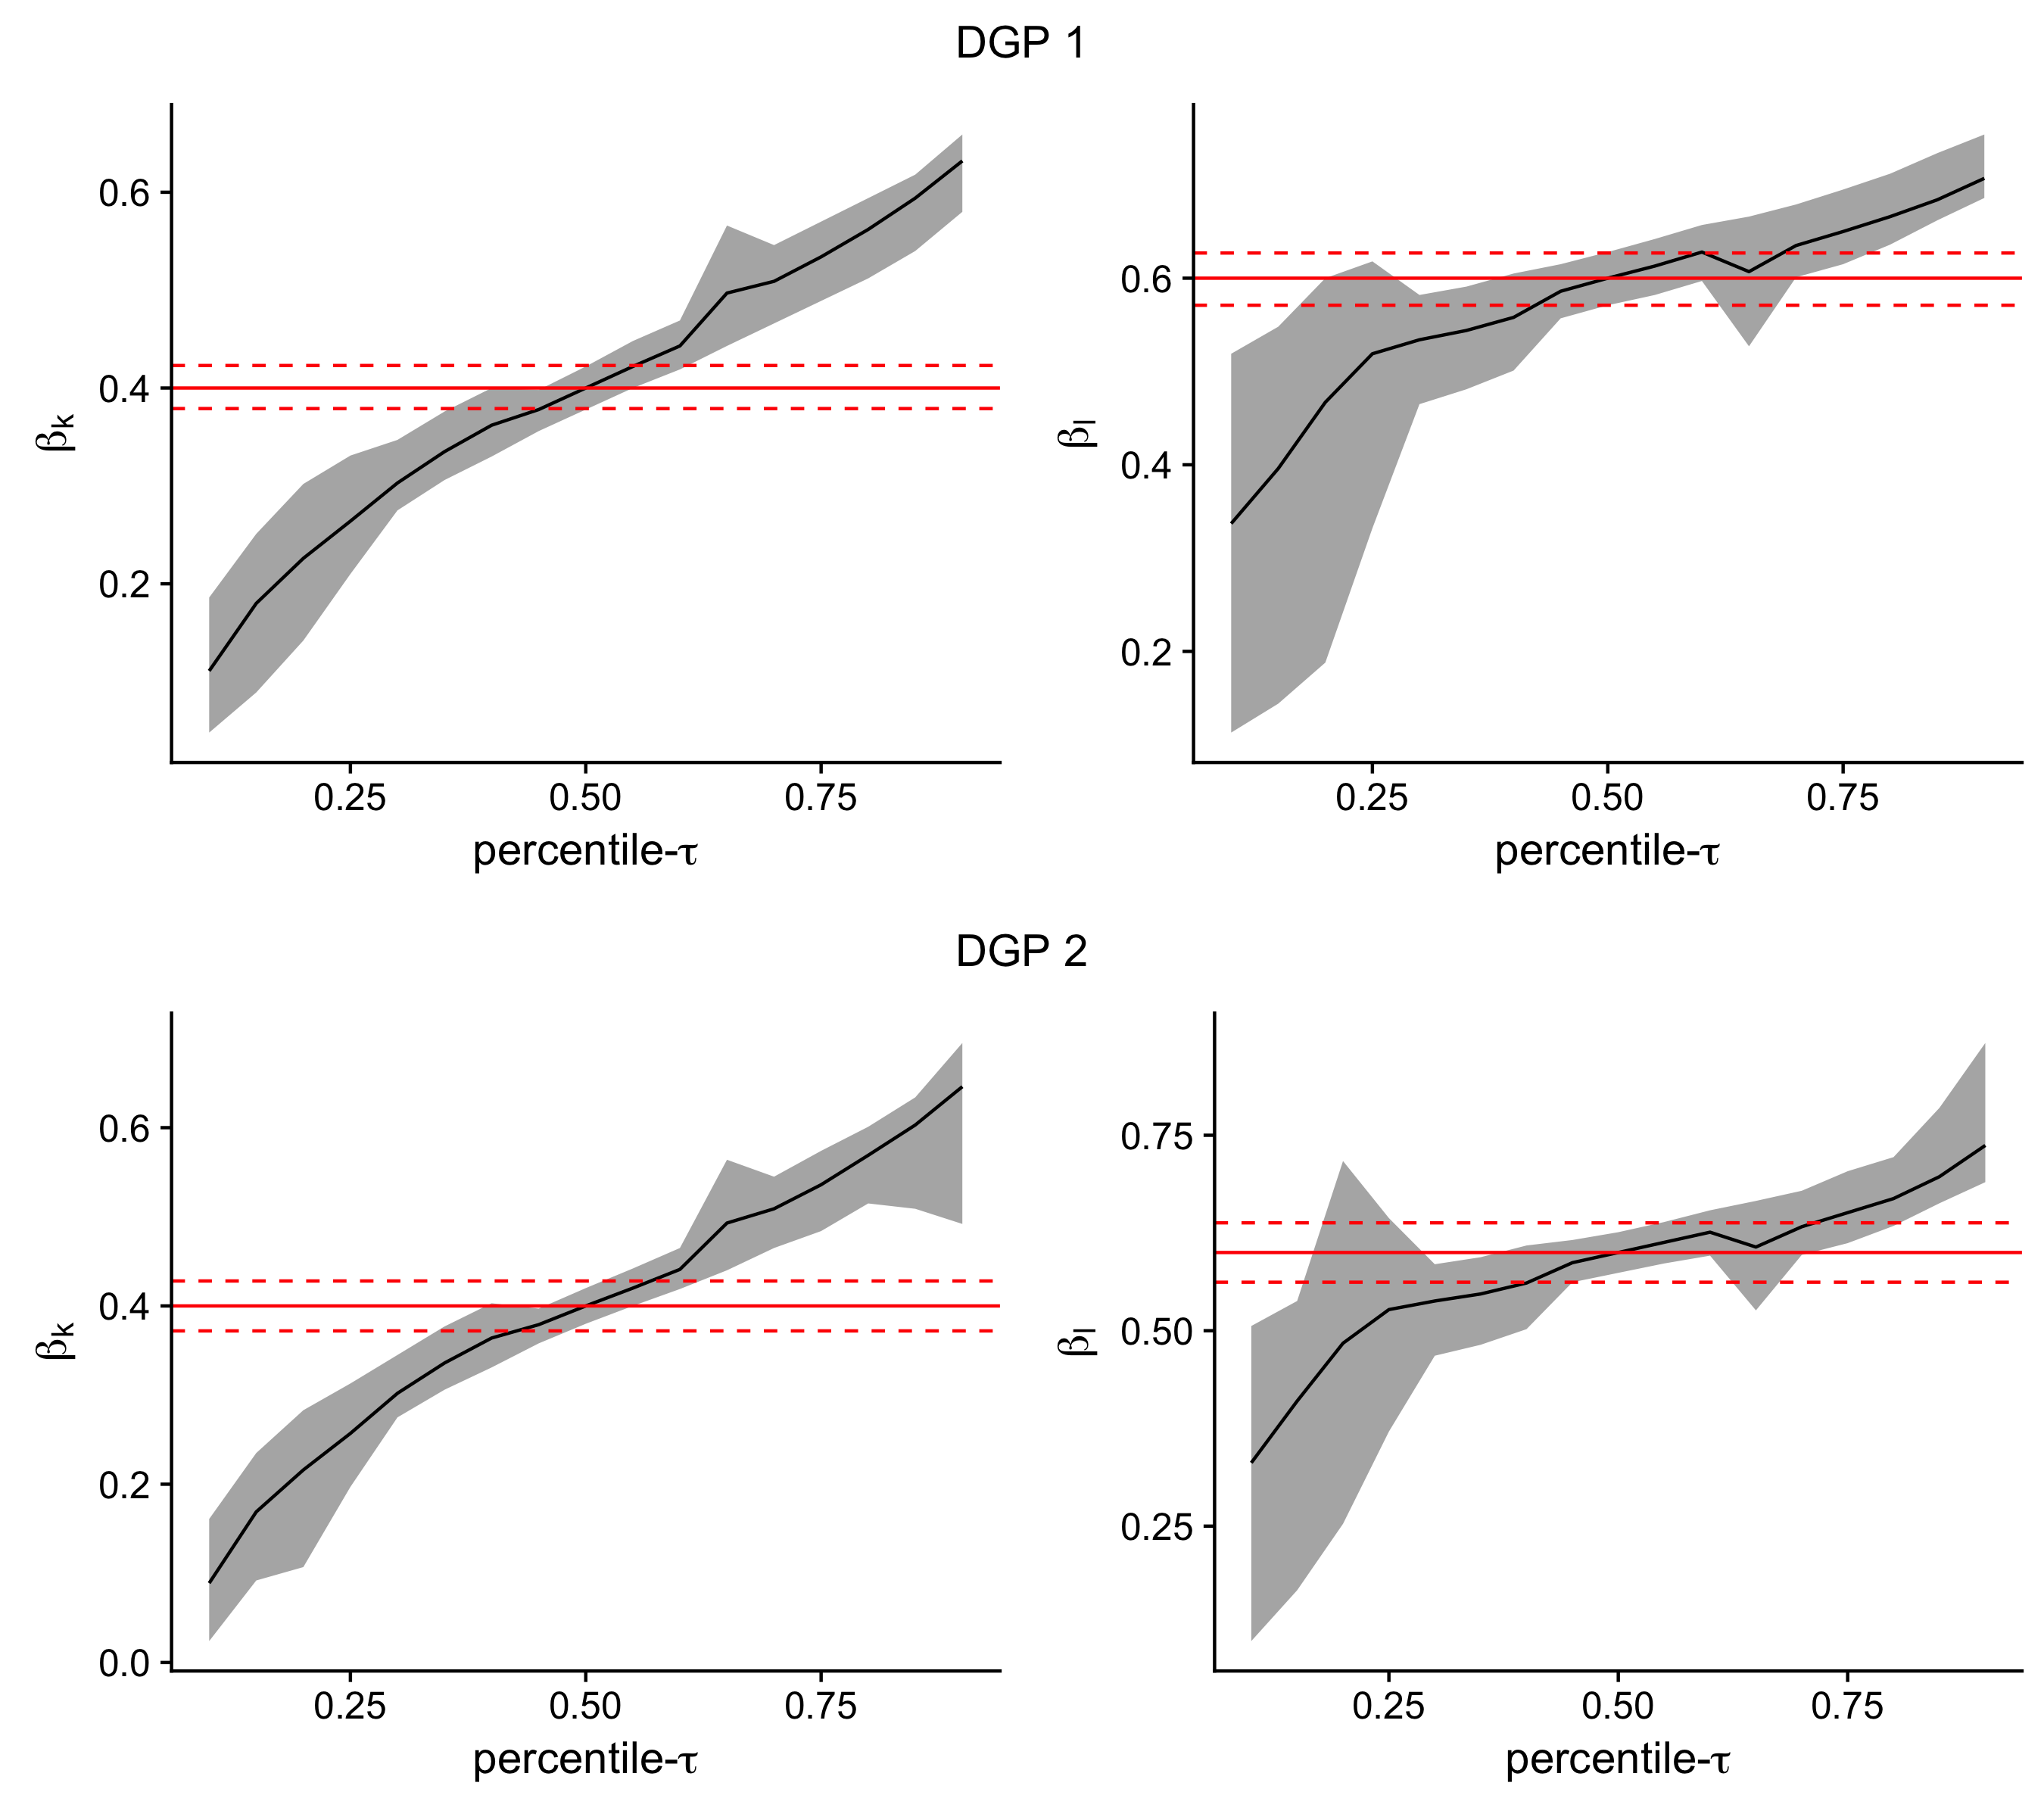
\includegraphics[width=12cm, height=6cm, keepaspectratio]{/Users/justindoty/Documents/Research/Dissertation/Production_QR_Proxy/Code/Monte_Carlo/ACF_Coefficient_Plot.png}
\end{figure}
\end{frame}

%----------------------------------------------------------------------------------

\begin{frame}
\frametitle{Monte Carlo Simulation 1}
\begin{figure}[H]
\centering
\caption{Simulated precision estimators of $\beta_{k}(\tau)$ and $\beta_{l}(\tau)$. Dotted line is ACF estimator}
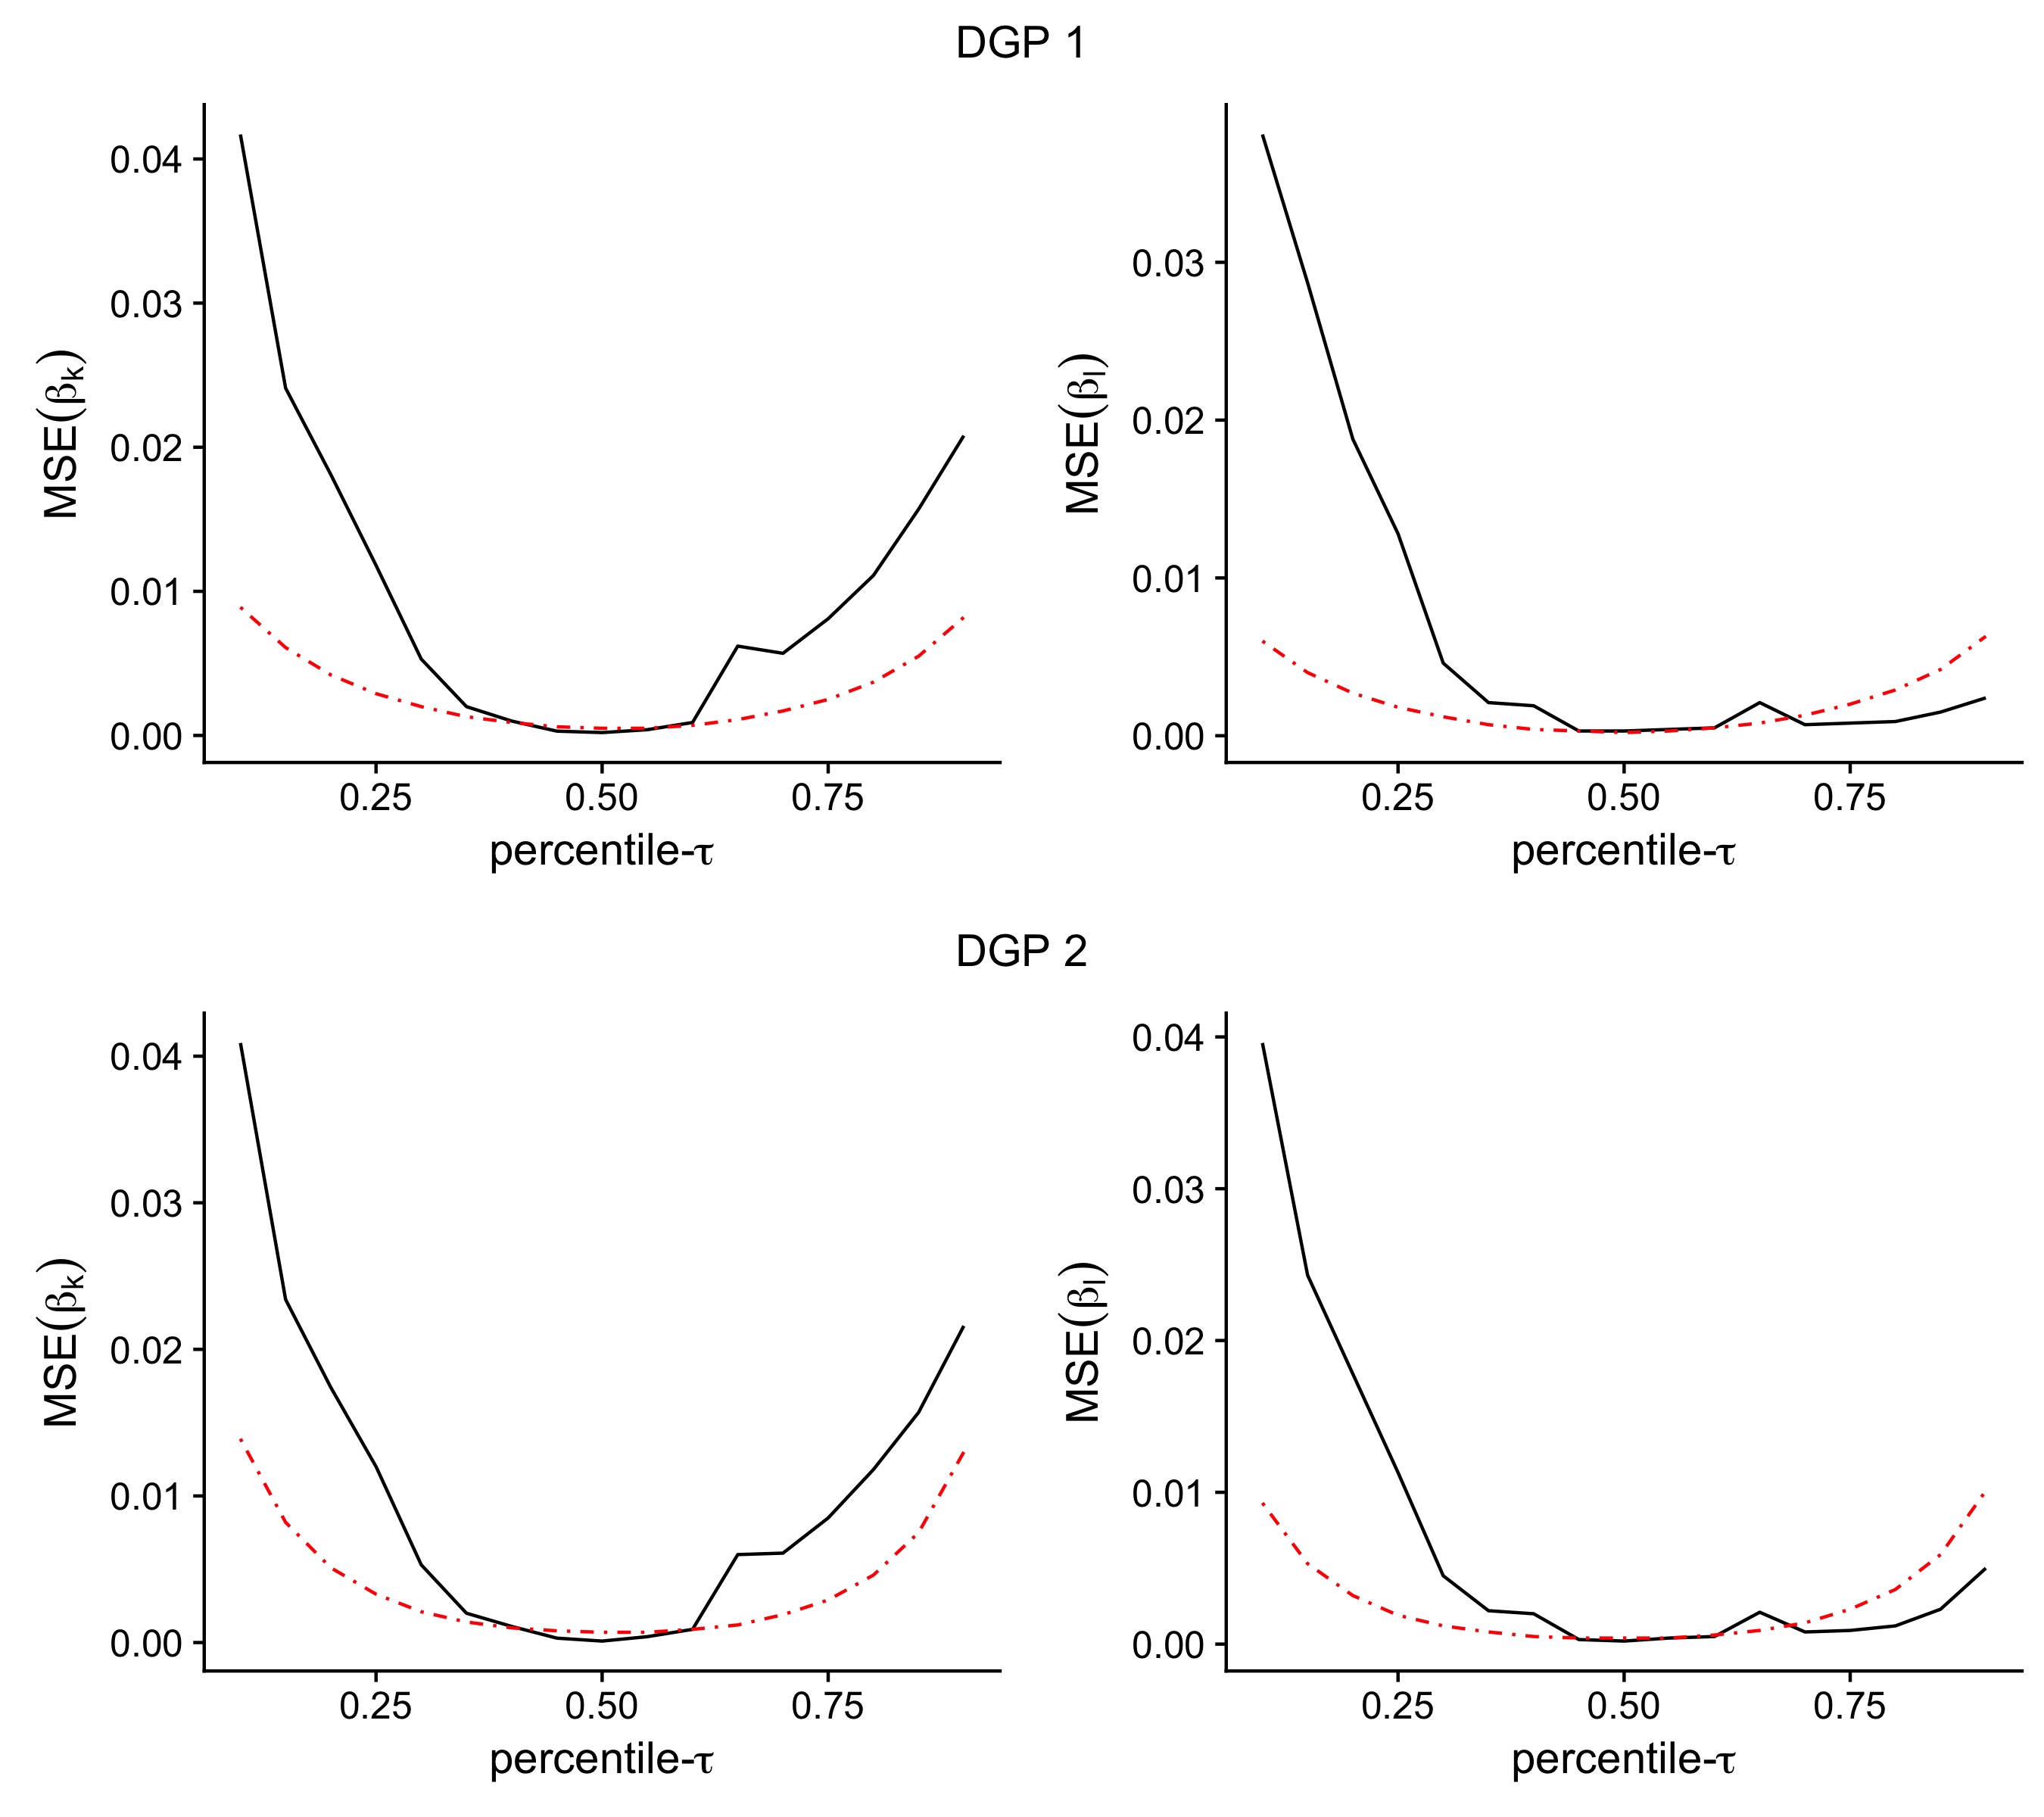
\includegraphics[width=12cm, height=6cm, keepaspectratio]{/Users/justindoty/Documents/Research/Dissertation/Production_QR_Proxy/Code/Monte_Carlo/ACF_MSE_Plot.png}
\end{figure}
\end{frame}
%----------------------------------------------------------------------------------

\begin{frame}
\frametitle{Monte Carlo: Simulation 2}
\begin{figure}[H]
\centering
\caption{Simulated estimators of $\beta_{k}(\tau)$ and $\beta_{l}(\tau)$. Dotted line is LP estimator}
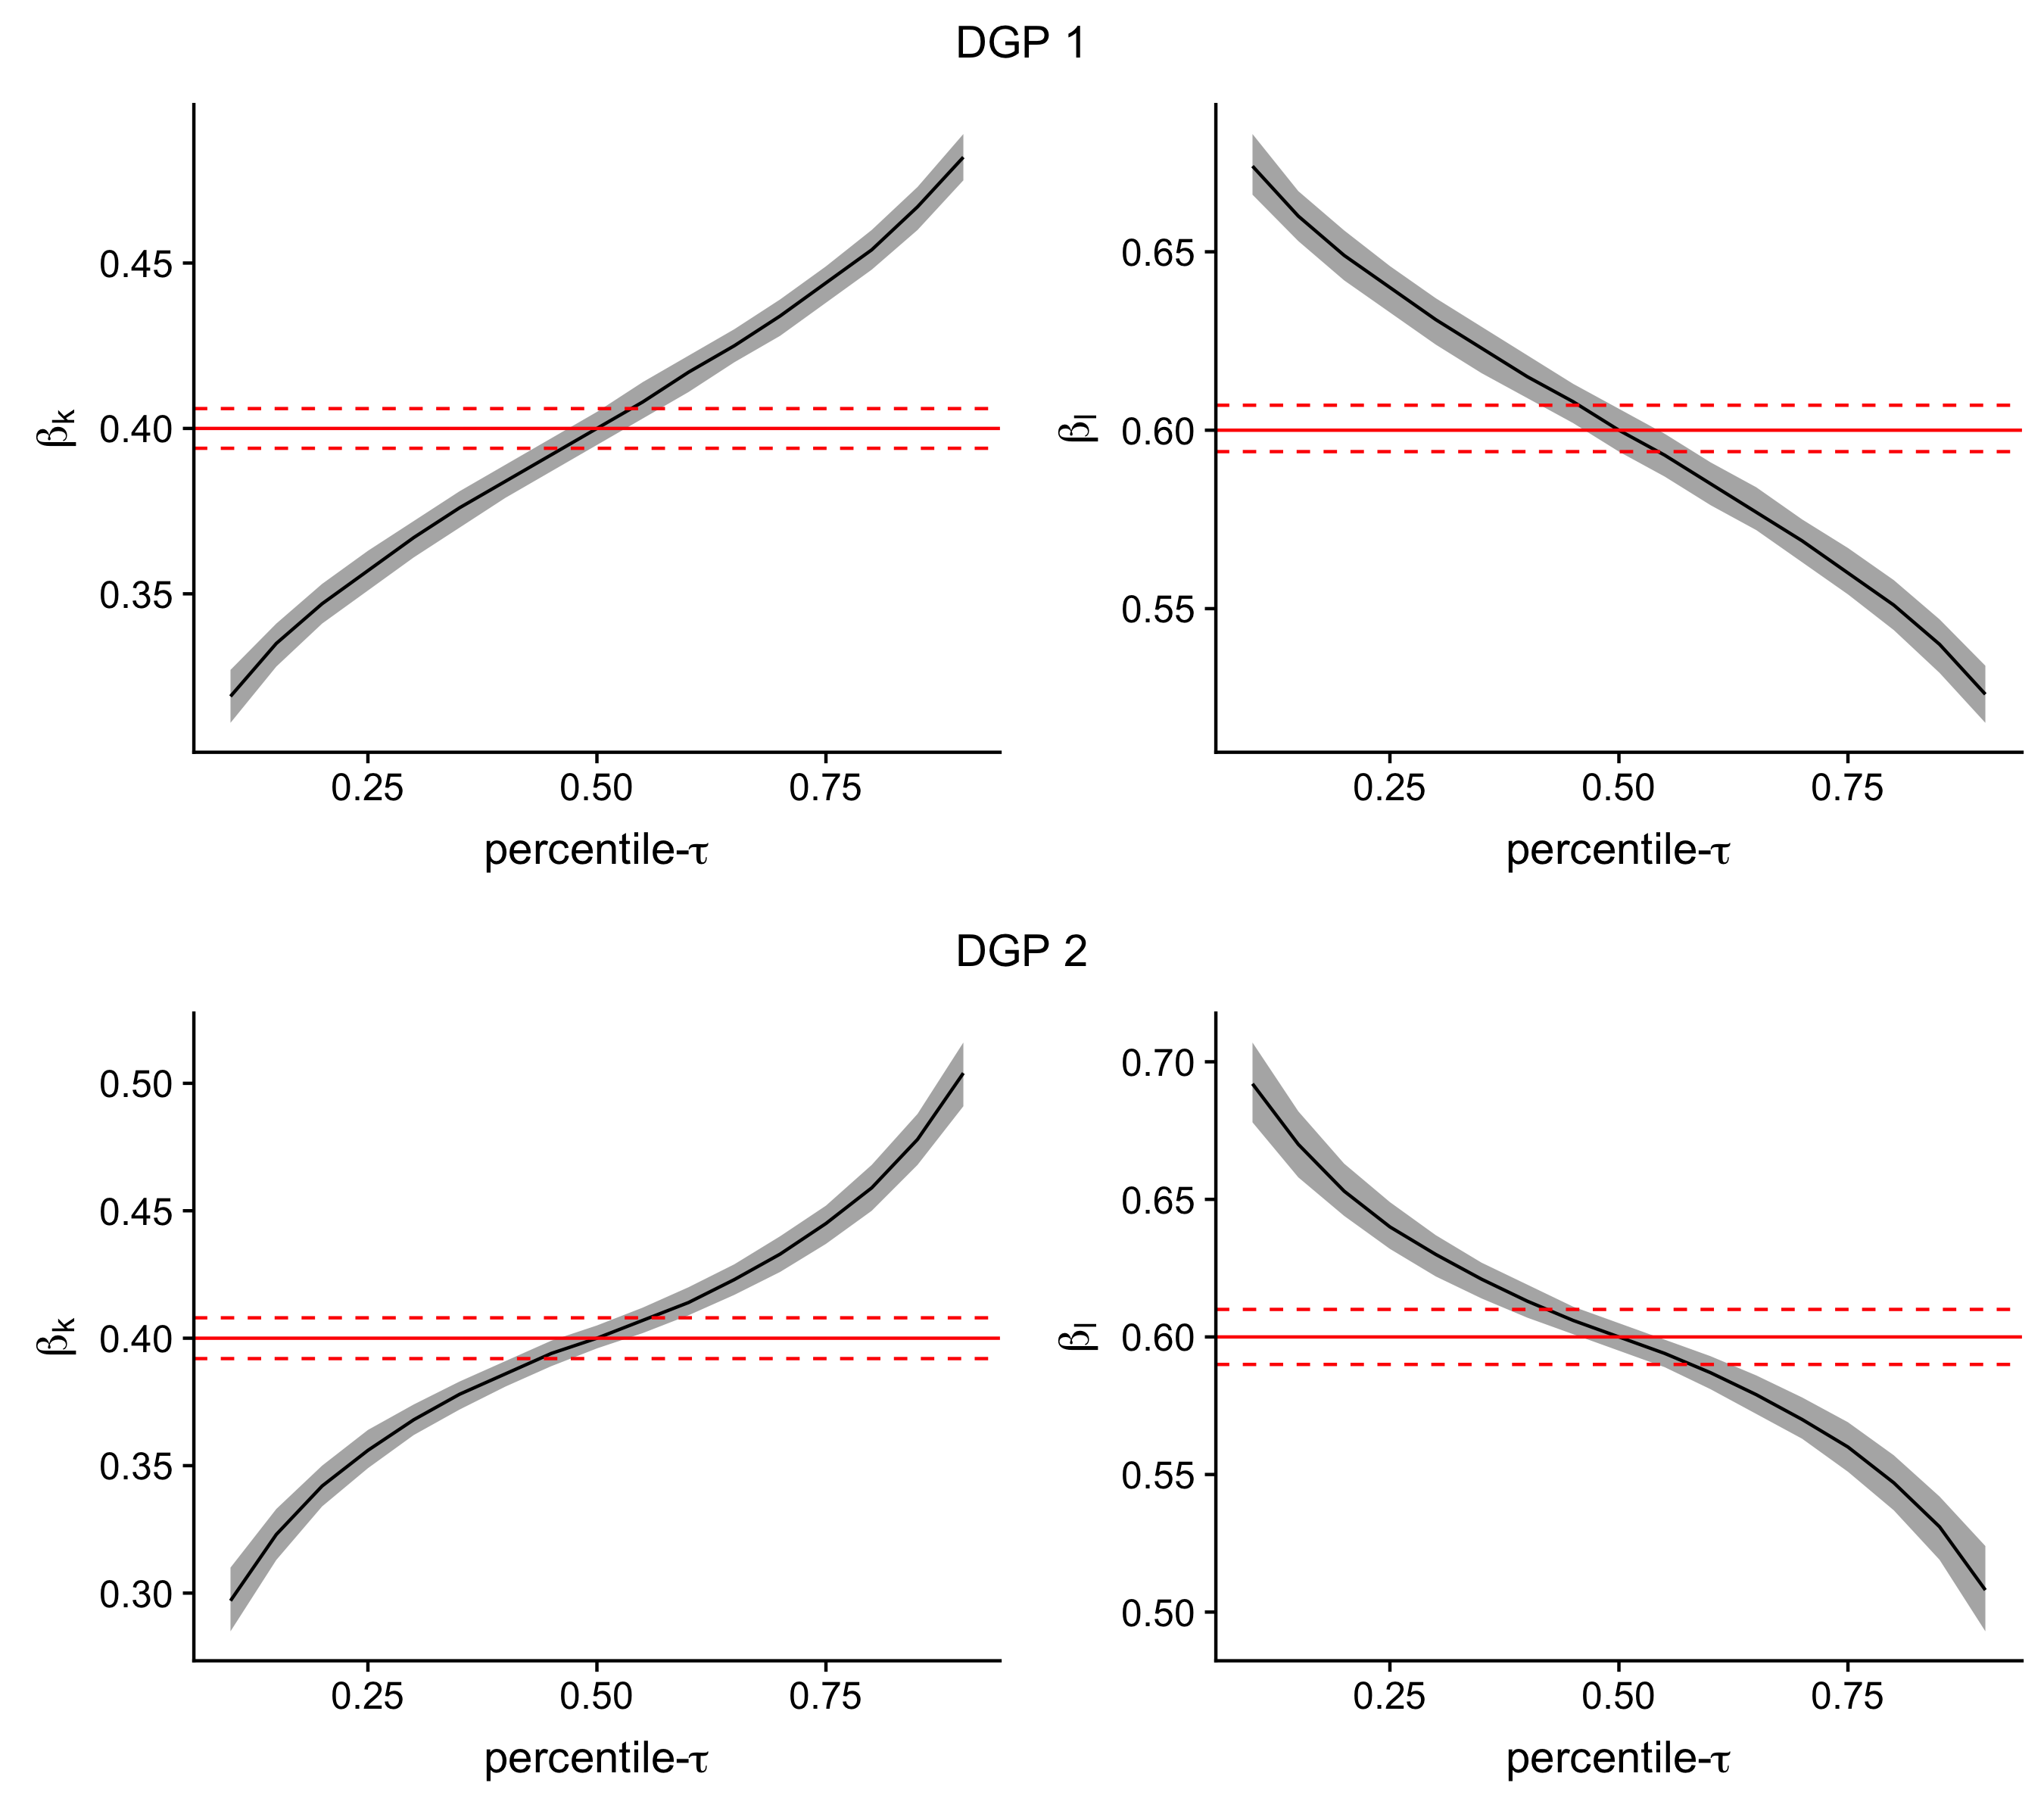
\includegraphics[width=12cm, height=6cm, keepaspectratio]{/Users/justindoty/Documents/Research/Dissertation/Production_QR_Proxy/Code/Monte_Carlo/LP_Coefficient_Plot.png}
\end{figure}
\end{frame}
%----------------------------------------------------------------------------------



\begin{frame}
\frametitle{Monte Carlo: Simulation 2}
\begin{figure}[H]
\centering
\caption{Simulated precision of estimators of $\beta_{k}(\tau)$ and $\beta_{l}(\tau)$. Dotted line is LP estimator}
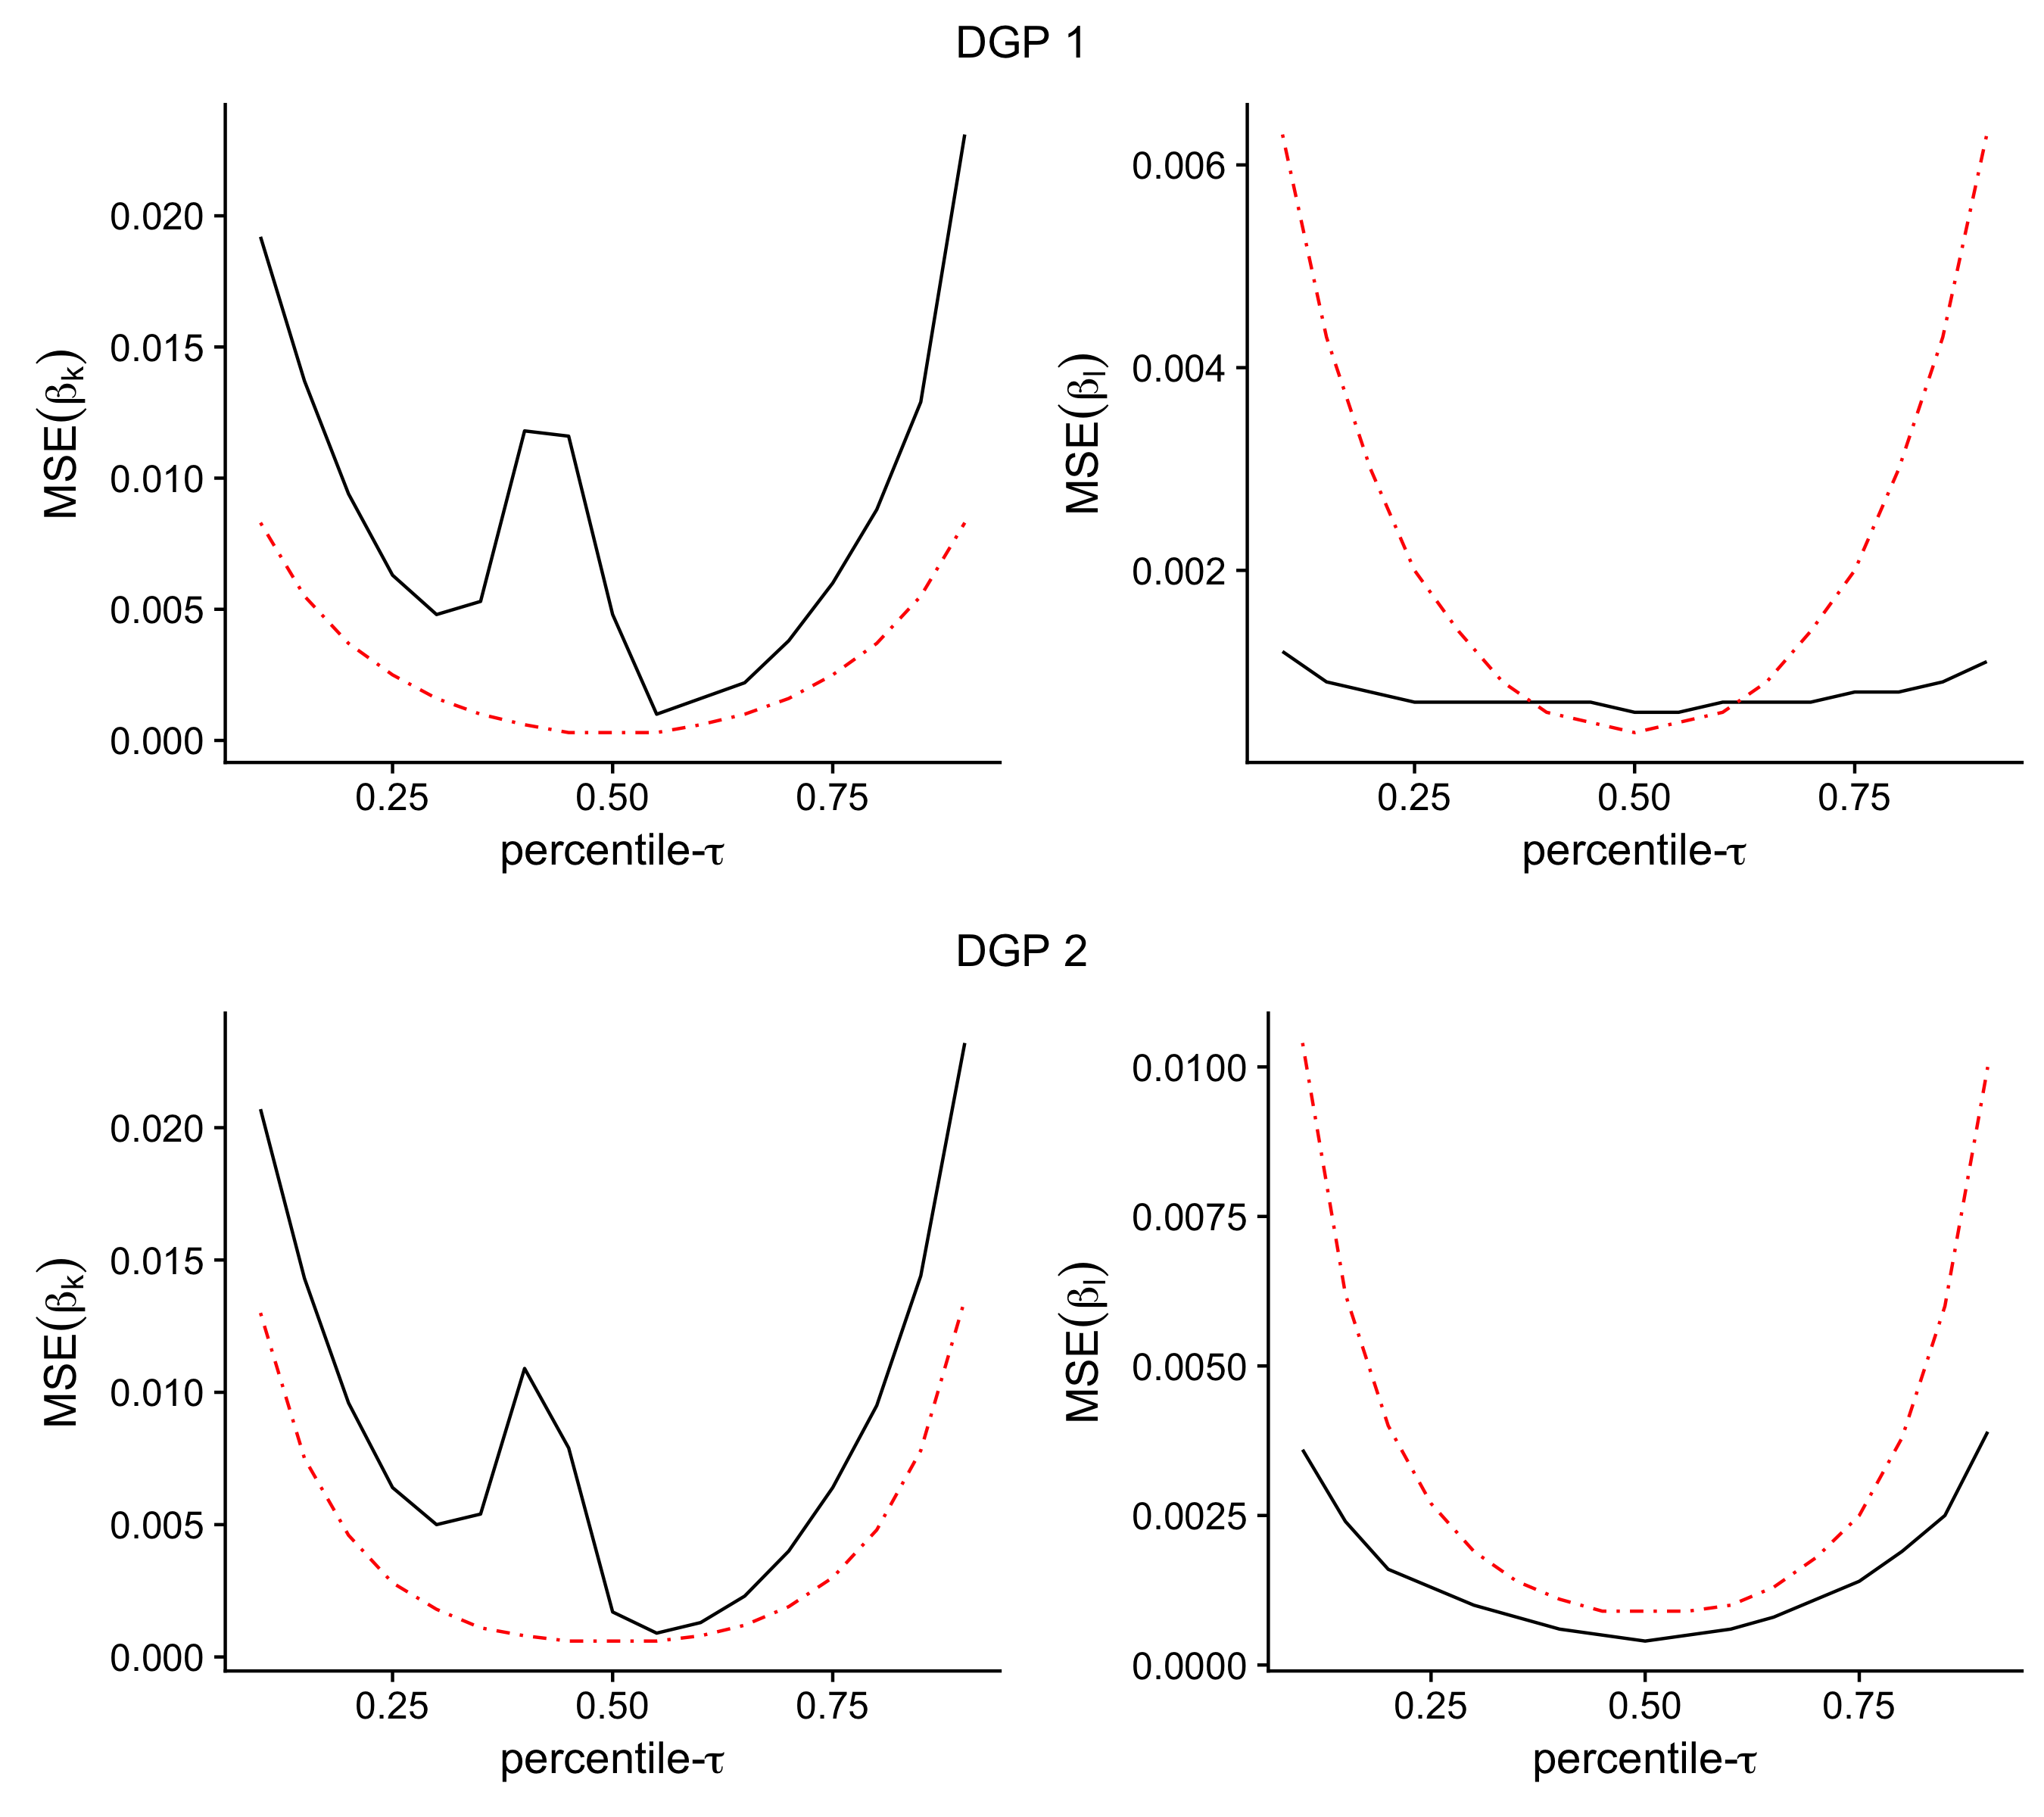
\includegraphics[width=12cm, height=6cm, keepaspectratio]{/Users/justindoty/Documents/Research/Dissertation/Production_QR_Proxy/Code/Monte_Carlo/LP_MSE_Plot.png}
\end{figure}
\end{frame}

%----------------------------------------------------------------------------------


\begin{frame}
\frametitle{Application}
\begin{itemize}
	\item We apply this estimator to three country manufacturing datasets: US, Chile, and Colombia
	\item The US data comes from Compustat which contains data on sales, capital expenditure, number of employees, and other items from firm's financial statements
	\item Compustat has been used in prior production function estimation although the data is of lower quality compared to the Census of Manufactures which is restricted data
	\item Our Compustat sample contains publicly traded manufacturing firms between 1961 and 2011
	\item Manufacturing data from Chile is collected by the Instituto Nacional de Estad\'{i}stica (INE) which contains plant level data from 1979 to 1996
	\item Manufacturing data from Colombia come from the manufacturing census which contains plant level data from 1981 to 1991 
	\item We only include the US results here due to time constraints
\end{itemize}
\end{frame}

%----------------------------------------------------------------------------------

\begin{frame}
\frametitle{US Manufacturing: Compustat}
\scriptsize
% latex table generated in R 3.4.1 by xtable 1.8-2 package
% Fri Mar  5 12:36:22 2021
\begin{table}[H]
\centering
\begin{tabular}{ccccccc}
  \hline\hline Industry (NAICS code) &   & 1st Qu. & Median & 3rd Qu. & Mean & sd \\ 
  \hline
31 (Total=3271) & Output & 19.05 & 20.24 & 21.57 & 20.3 & 1.77 \\ 
   & Capital & 18.66 & 20.37 & 21.76 & 20.19 & 2.12 \\ 
   & Labor & 17.42 & 19.08 & 20.61 & 19.02 & 2.21 \\ 
   & Materials & 17.96 & 19.59 & 21.15 & 19.54 & 2.21 \\ 
  32 (Total=7207) & Output & 15.67 & 17.04 & 18.51 & 17.01 & 2.05 \\ 
   & Capital & 15.65 & 17.51 & 19.13 & 17.31 & 2.41 \\ 
   & Labor & 14.44 & 16.01 & 17.57 & 16.01 & 2.29 \\ 
   & Materials & 14.89 & 16.53 & 18.25 & 16.52 & 2.37 \\ 
  33 (Total=13978) & Output & 7.38 & 8.58 & 9.8 & 8.5 & 1.67 \\ 
   & Capital & 6.67 & 8.29 & 9.74 & 8.15 & 1.95 \\ 
   & Labor & 6.01 & 7.42 & 8.91 & 7.48 & 1.93 \\ 
   & Materials & 6.33 & 7.82 & 9.29 & 7.82 & 1.95 \\ 
  All (Total=24456) & Output & 18.58 & 19.78 & 21.23 & 19.85 & 1.79 \\ 
   & Capital & 18.14 & 19.86 & 21.26 & 19.67 & 2.16 \\ 
   & Labor & 16.98 & 18.59 & 20.13 & 18.56 & 2.17 \\ 
   & Materials & 17.49 & 19.12 & 20.66 & 19.06 & 2.2 \\ 
   \hline
\end{tabular}
\end{table}

\end{frame}
%----------------------------------------------------------------------------------

\begin{frame}
\frametitle{US Manufacturing: Compustat}
\scriptsize
% latex table generated in R 3.4.1 by xtable 1.8-2 package
% Mon Sep 14 17:49:58 2020
\begin{table}[ht]
\centering
\caption{Coefficient Estimates and Standard Errors for US Manufacturing Firms} 
\begin{tabular}{cccccccc}
  \hline\hline & & \multicolumn{2}{c}{Capital}  & \multicolumn{2}{c}{Labor} & \multicolumn{2}{c}{Returns to Scale} \\ \cmidrule(lr){3-4} \cmidrule(lr){5-6} \cmidrule(lr){7-8}Industry (NAICS code) & $\tau$ & Coef. & s.e. & Coef. & s.e. & Coef. & s.e \\ 
  \hline
31 & 0.10 & 0.406 & 0.2415 & 0.612 & 0.0312 & 1.018 & 0.2416 \\ 
   & 0.25 & 0.385 & 0.2076 & 0.551 & 0.0348 & 0.937 & 0.2071 \\ 
   & 0.50 & 0.440 & 0.1921 & 0.478 & 0.0368 & 0.917 & 0.1973 \\ 
   & 0.75 & 0.394 & 0.2358 & 0.446 & 0.0364 & 0.839 & 0.2362 \\ 
  32 & 0.10 & 0.468 & 0.2527 & 0.692 & 0.0449 & 1.160 & 0.2590 \\ 
   & 0.25 & 0.521 & 0.1519 & 0.630 & 0.0306 & 1.150 & 0.1554 \\ 
   & 0.50 & 0.358 & 0.2937 & 0.587 & 0.0254 & 0.945 & 0.2946 \\ 
   & 0.75 & 0.325 & 0.2807 & 0.548 & 0.0235 & 0.872 & 0.2861 \\ 
  33 & 0.10 & 0.464 & 0.3609 & 0.214 & 0.0579 & 0.678 & 0.3570 \\ 
   & 0.25 & 0.313 & 0.1242 & 0.358 & 0.0391 & 0.671 & 0.1289 \\ 
   & 0.50 & 0.513 & 0.1026 & 0.449 & 0.0283 & 0.961 & 0.1104 \\ 
   & 0.75 & 0.475 & 0.2916 & 0.472 & 0.0199 & 0.946 & 0.2905 \\ 
  All & 0.10 & 0.698 & 0.2995 & 0.366 & 0.0351 & 1.064 & 0.3021 \\ 
   & 0.25 & 0.208 & 0.1799 & 0.414 & 0.0234 & 0.622 & 0.1831 \\ 
   & 0.50 & 0.451 & 0.0829 & 0.475 & 0.0193 & 0.926 & 0.0864 \\ 
   & 0.75 & 0.586 & 0.1988 & 0.486 & 0.0161 & 1.072 & 0.1994 \\ 
   \hline
\end{tabular}
\end{table}

\end{frame}

%----------------------------------------------------------------------------------
\begin{frame}
\frametitle{US Manufacturing: Compustat}
\begin{figure}[ht]
\centering
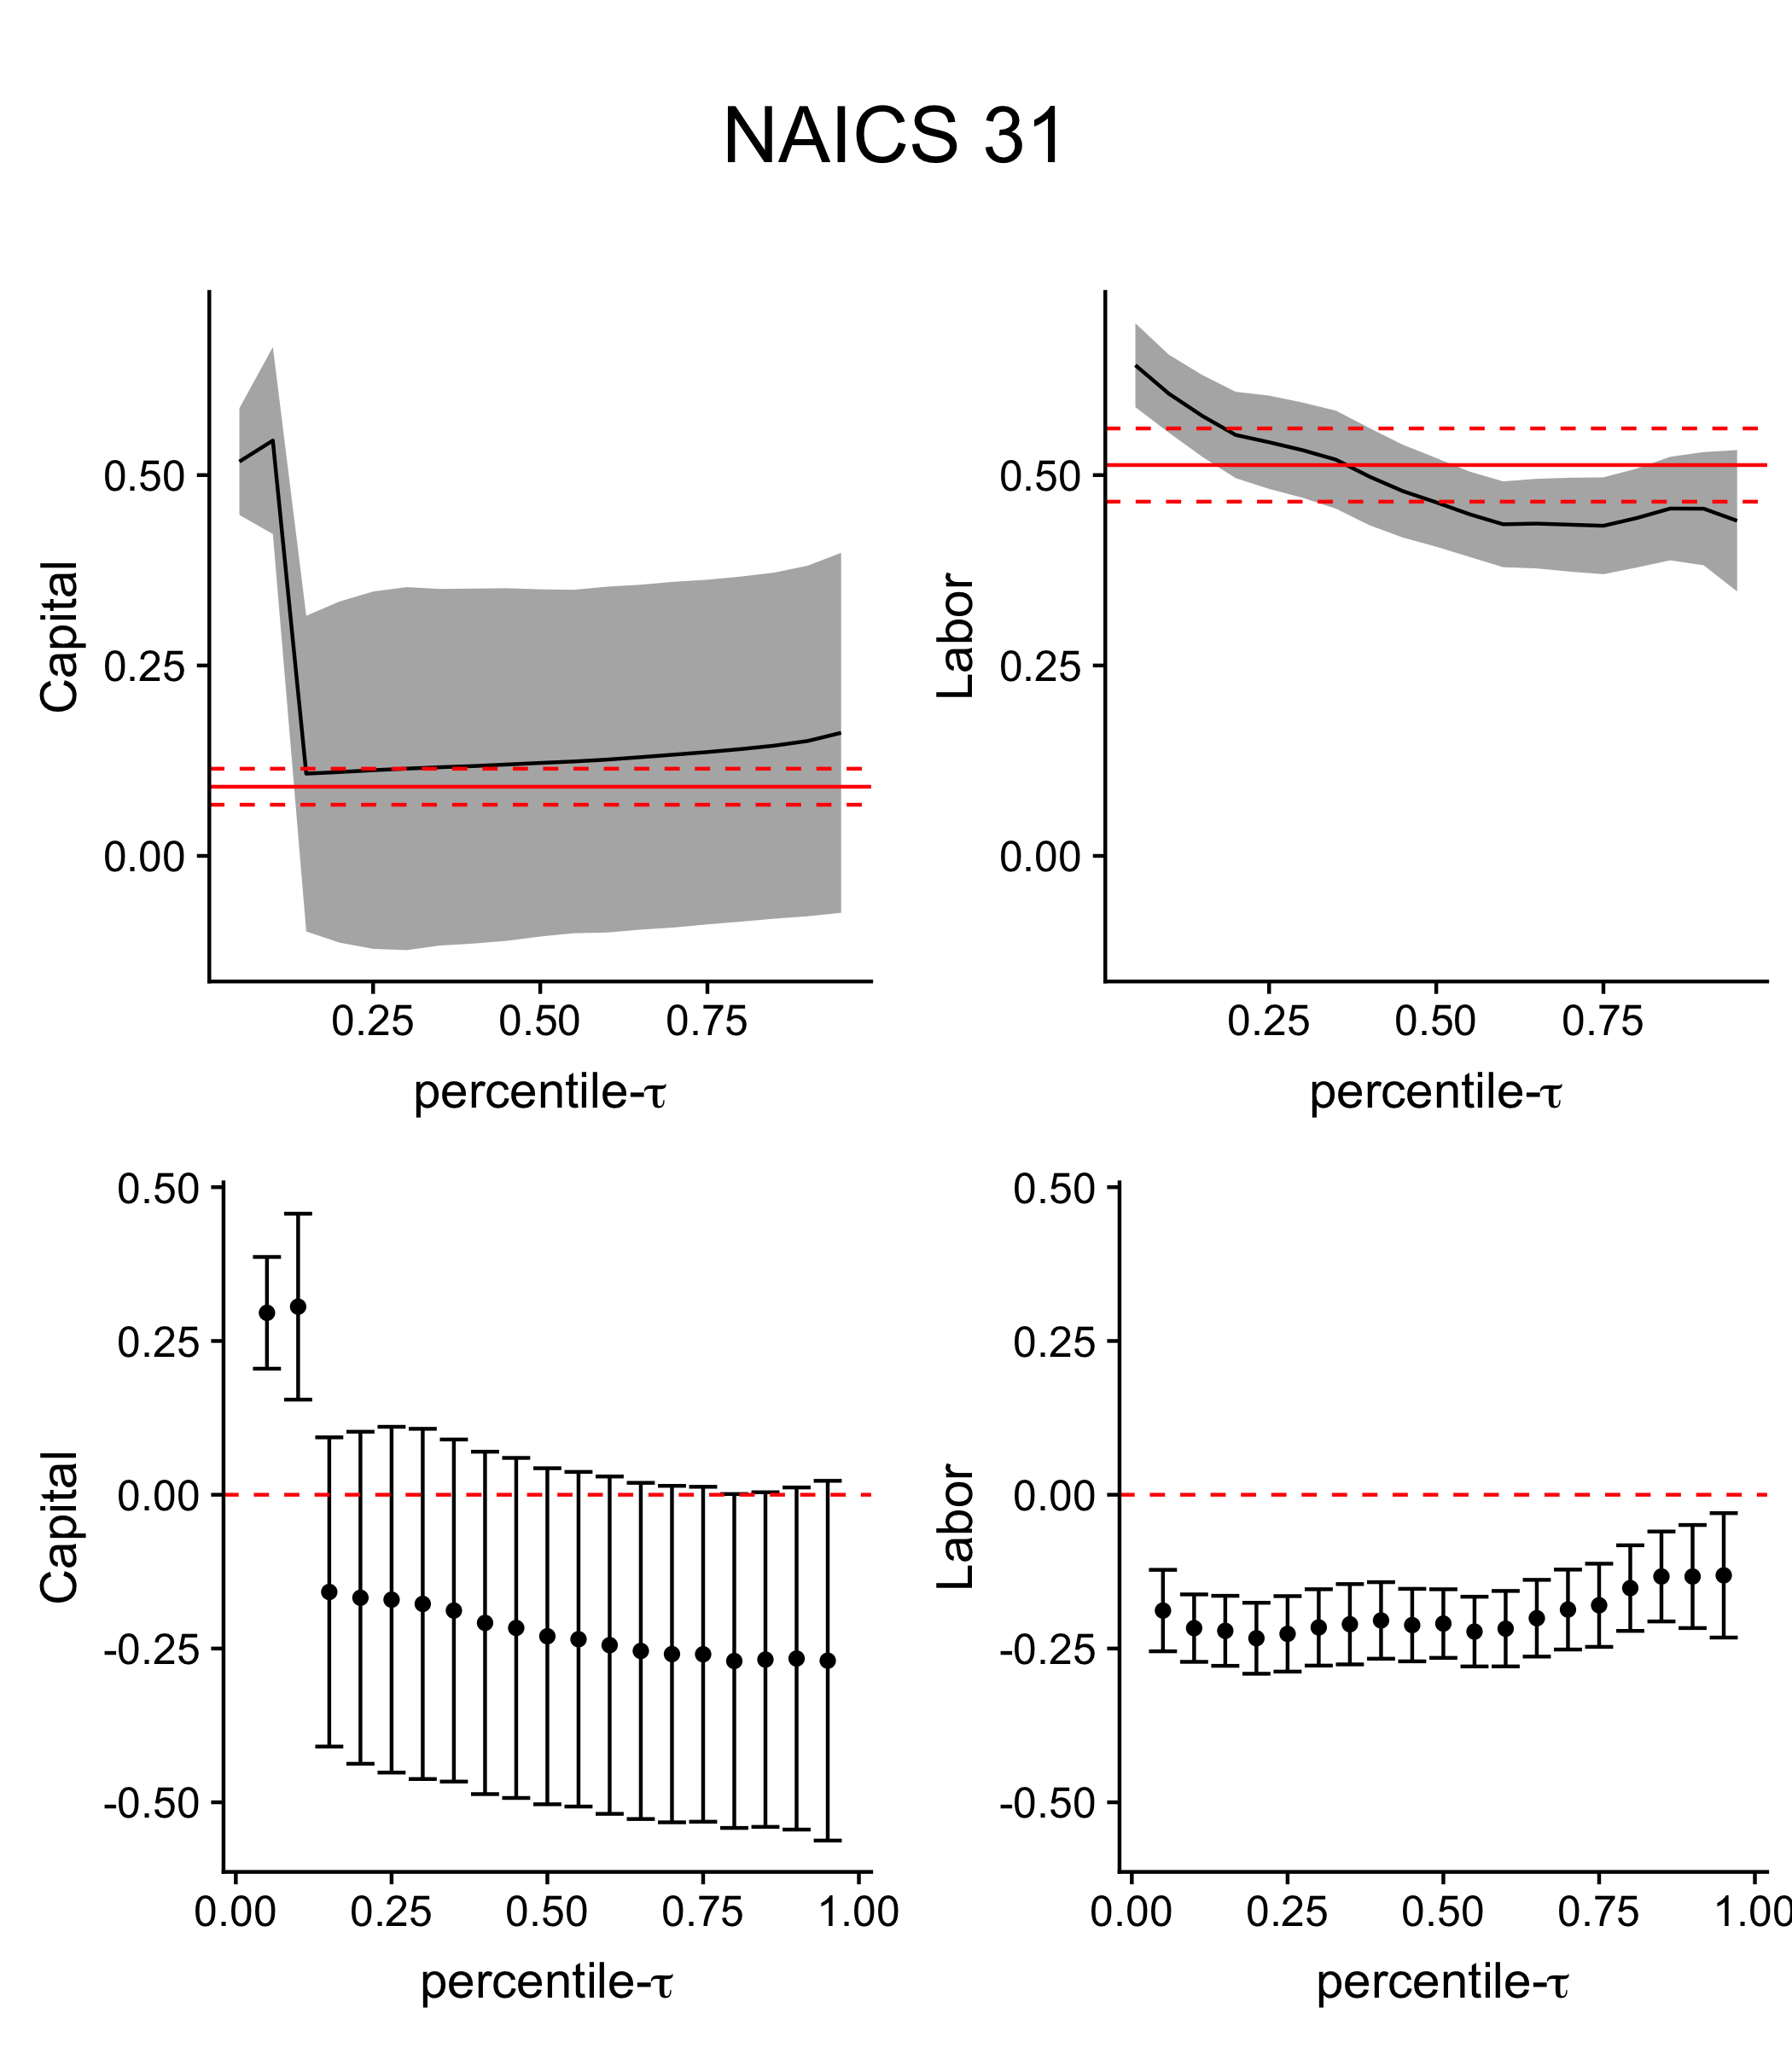
\includegraphics[width=6cm, height=6cm]{/Users/justindoty/Documents/Research/Dissertation/Production_QR_Proxy/Code/Empirical/US/Plots/Coef_Plot_NAICS_31.png}
\caption{Estimated values of production function coefficients and their 90\% confidence interval. The plots on the LHS are the QLP and LP estimates. The plots on the RHS are quantile regression and OLS estimates}
\end{figure}
\end{frame}

%----------------------------------------------------------------------------------
\begin{frame}
\frametitle{US Manufacturing: Compustat}
\begin{figure}[ht]
\centering
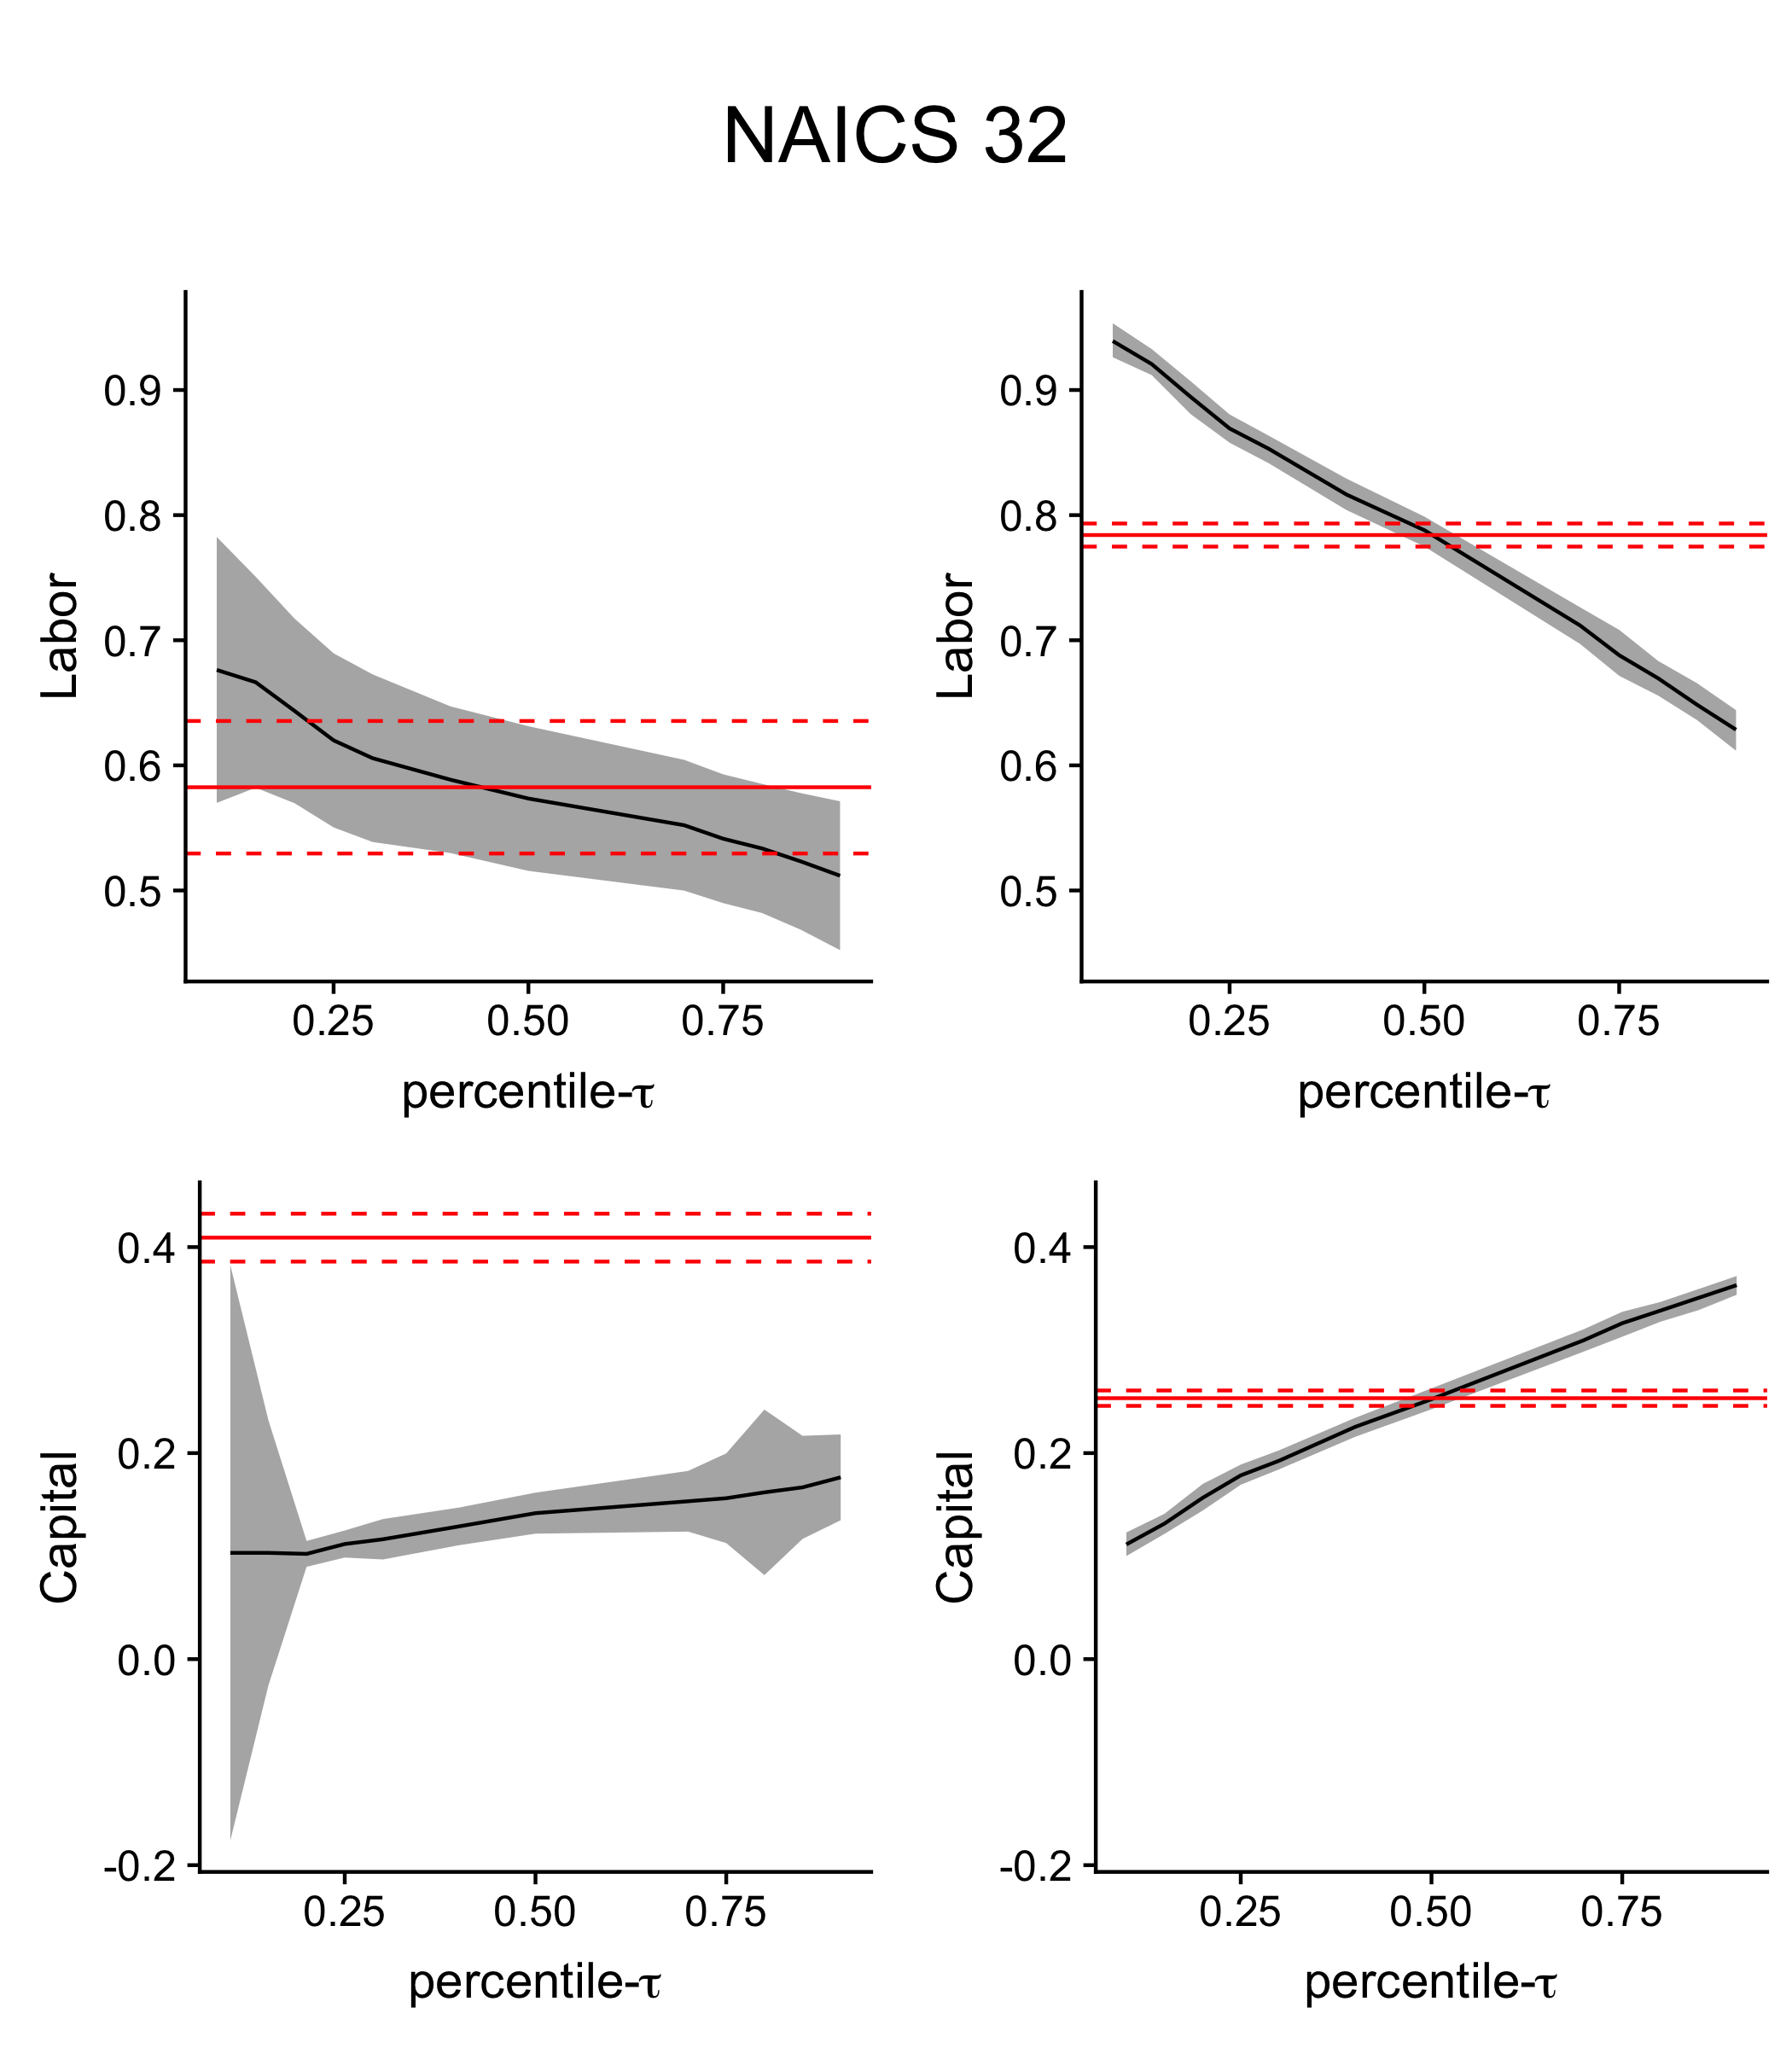
\includegraphics[width=6cm, height=6cm]{/Users/justindoty/Documents/Research/Dissertation/Production_QR_Proxy/Code/Empirical/US/Plots/Coef_Plot_NAICS_32.png}
\caption{Estimated values of production function coefficients and their 90\% confidence interval. The plots on the LHS are the QLP and LP estimates. The plots on the RHS are quantile regression and OLS estimates}
\end{figure}
\end{frame}

%----------------------------------------------------------------------------------
\begin{frame}
\frametitle{US Manufacturing: Compustat}
\begin{figure}[ht]
\centering
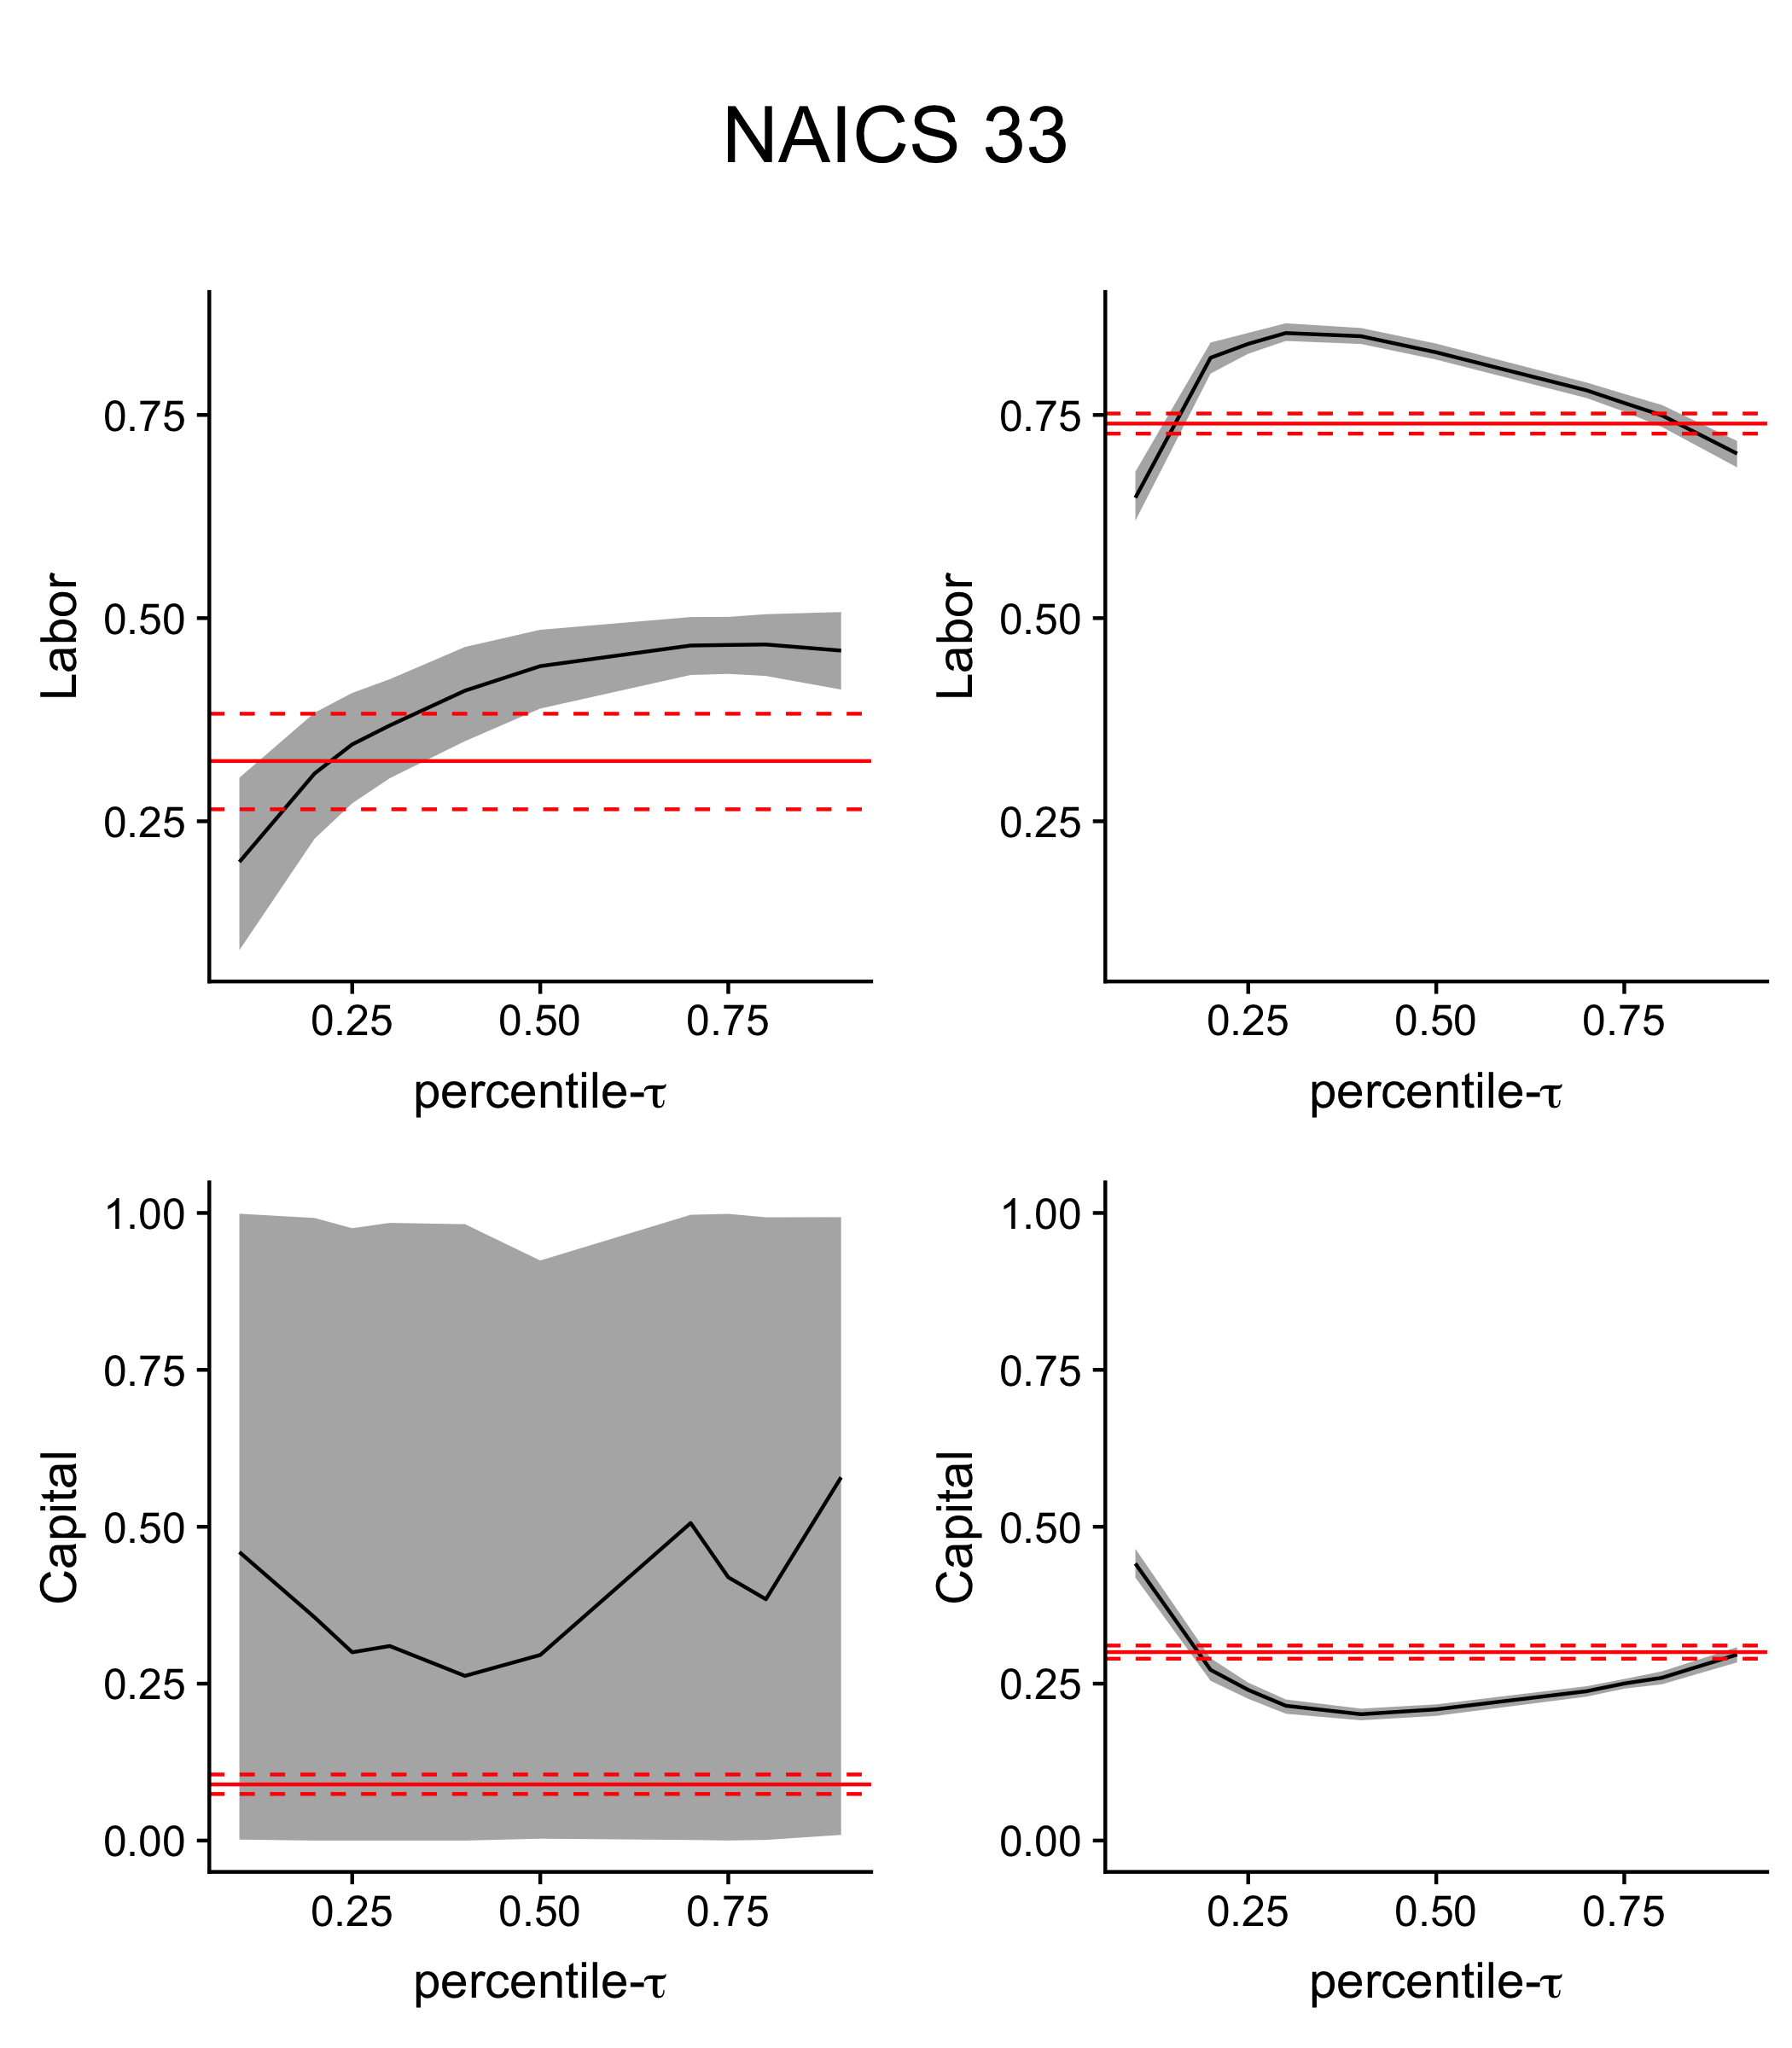
\includegraphics[width=6cm, height=6cm]{/Users/justindoty/Documents/Research/Dissertation/Production_QR_Proxy/Code/Empirical/US/Plots/Coef_Plot_NAICS_33.png}
\caption{Estimated values of production function coefficients and their 90\% confidence interval. The plots on the LHS are the QLP and LP estimates. The plots on the RHS are quantile regression and OLS estimates}
\end{figure}
\end{frame}

%----------------------------------------------------------------------------------
\begin{frame}
\frametitle{US Manufacturing: Compustat}
\begin{figure}[ht]
\centering
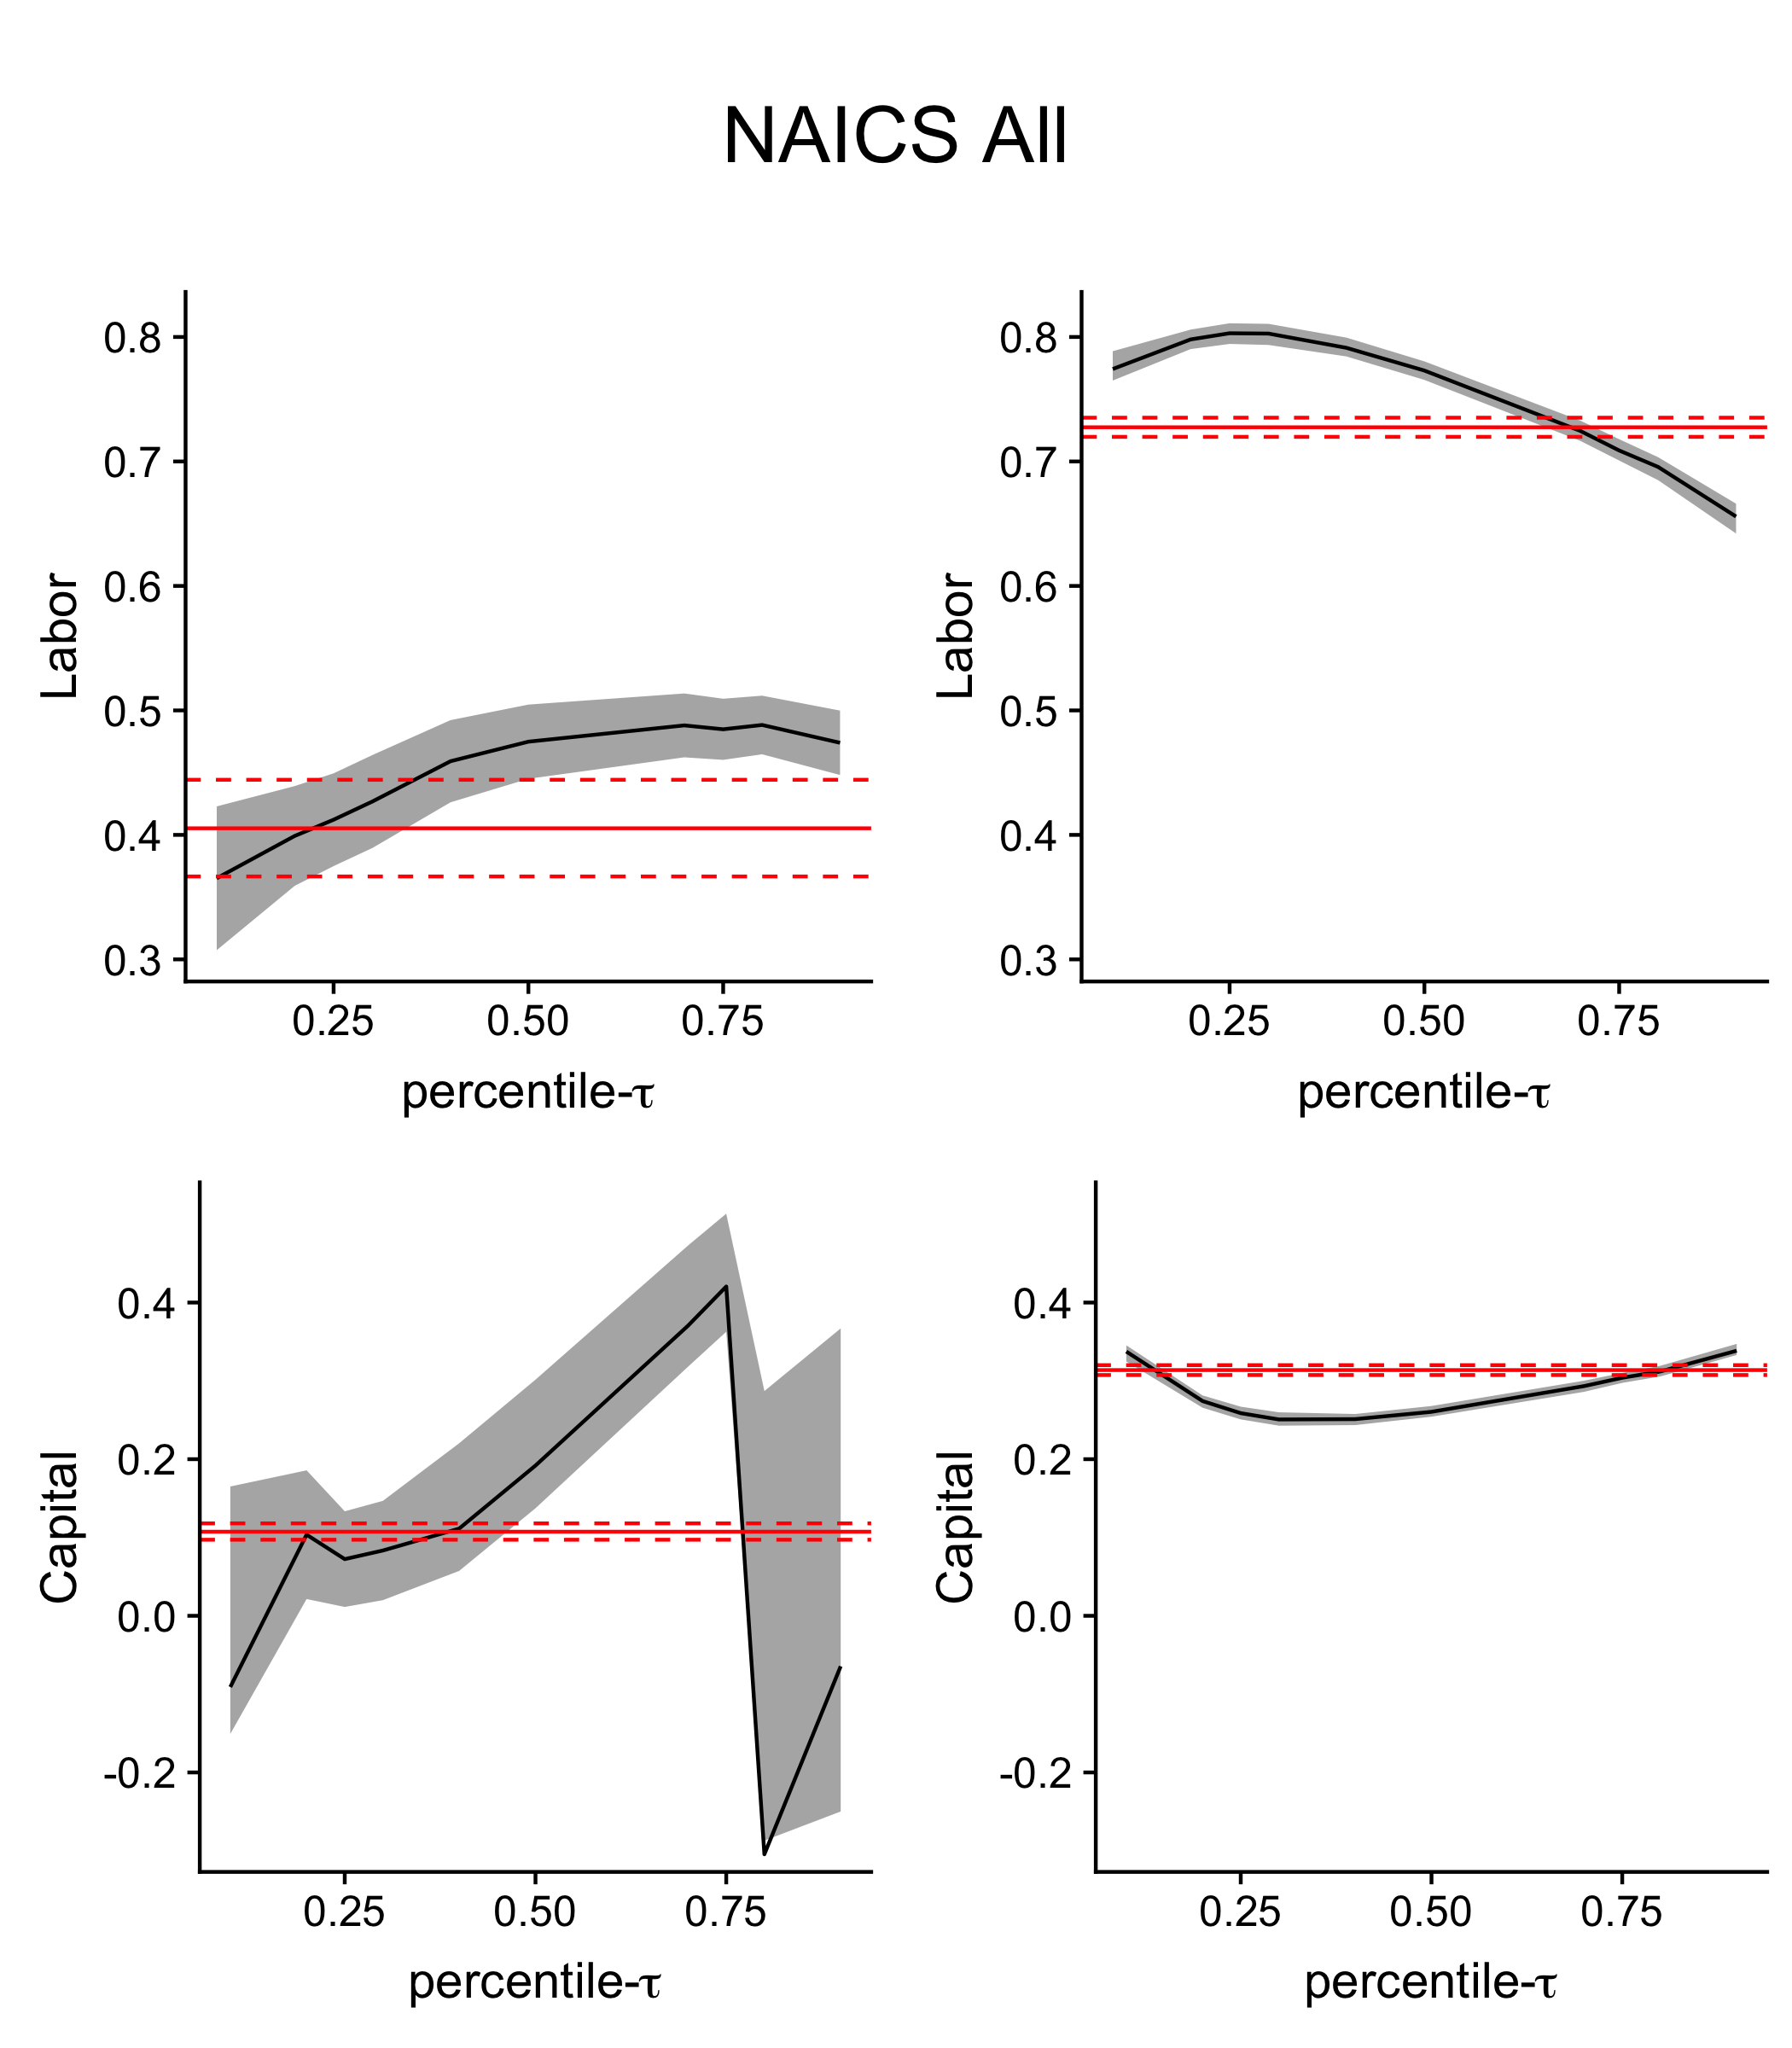
\includegraphics[width=6cm, height=6cm]{/Users/justindoty/Documents/Research/Dissertation/Production_QR_Proxy/Code/Empirical/US/Plots/Coef_Plot_NAICS_All.png}
\caption{Estimated values of production function coefficients and their 90\% confidence interval. The plots on the LHS are the QLP and LP estimates. The plots on the RHS are quantile regression and OLS estimates}
\end{figure}
\end{frame}

%----------------------------------------------------------------------------------
\begin{frame}
\frametitle{US Manufacturing: Compustat}
\begin{figure}[ht]
\centering
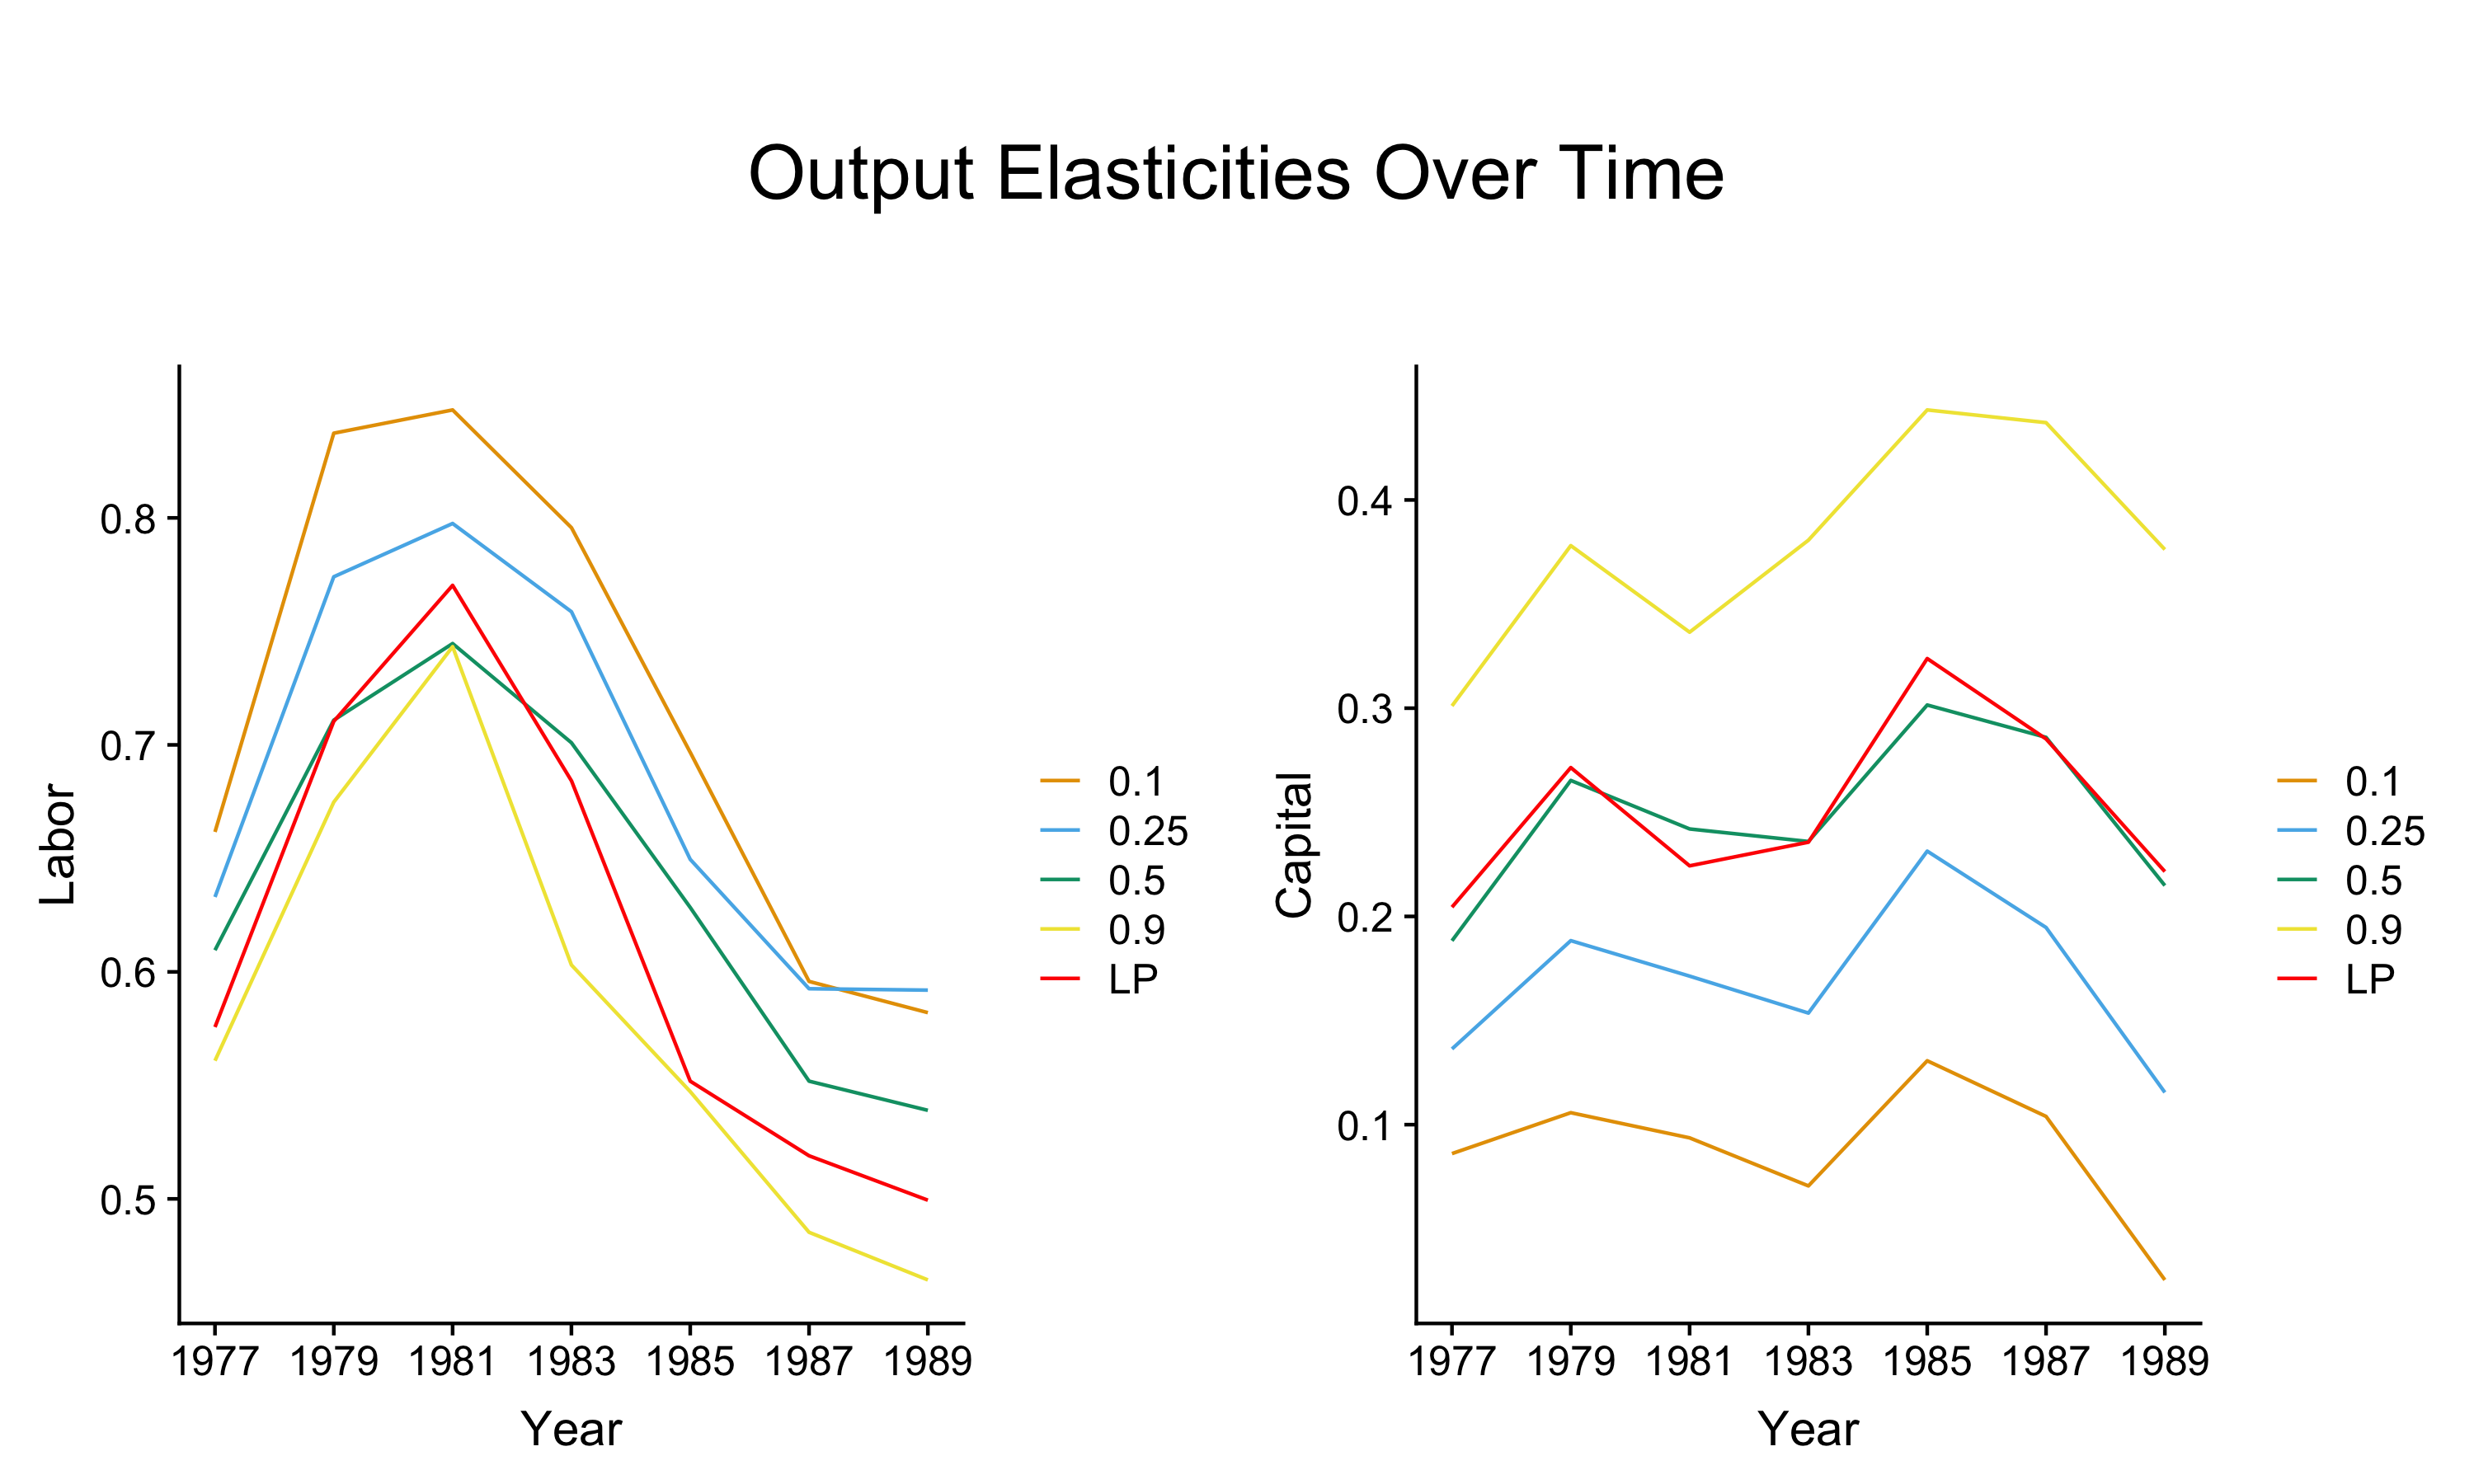
\includegraphics[width=11cm, height=6cm]{/Users/justindoty/Documents/Research/Dissertation/Production_QR_Proxy/Code/Empirical/US/Plots/Time_Plot.png}
\caption{Estimated values of production function coefficients over time. Estimated at 5 year intervals}
\end{figure}
\end{frame}

%----------------------------------------------------------------------------------
\begin{frame}
\frametitle{US Manufacturing: Compustat}
\begin{figure}[ht]
\centering
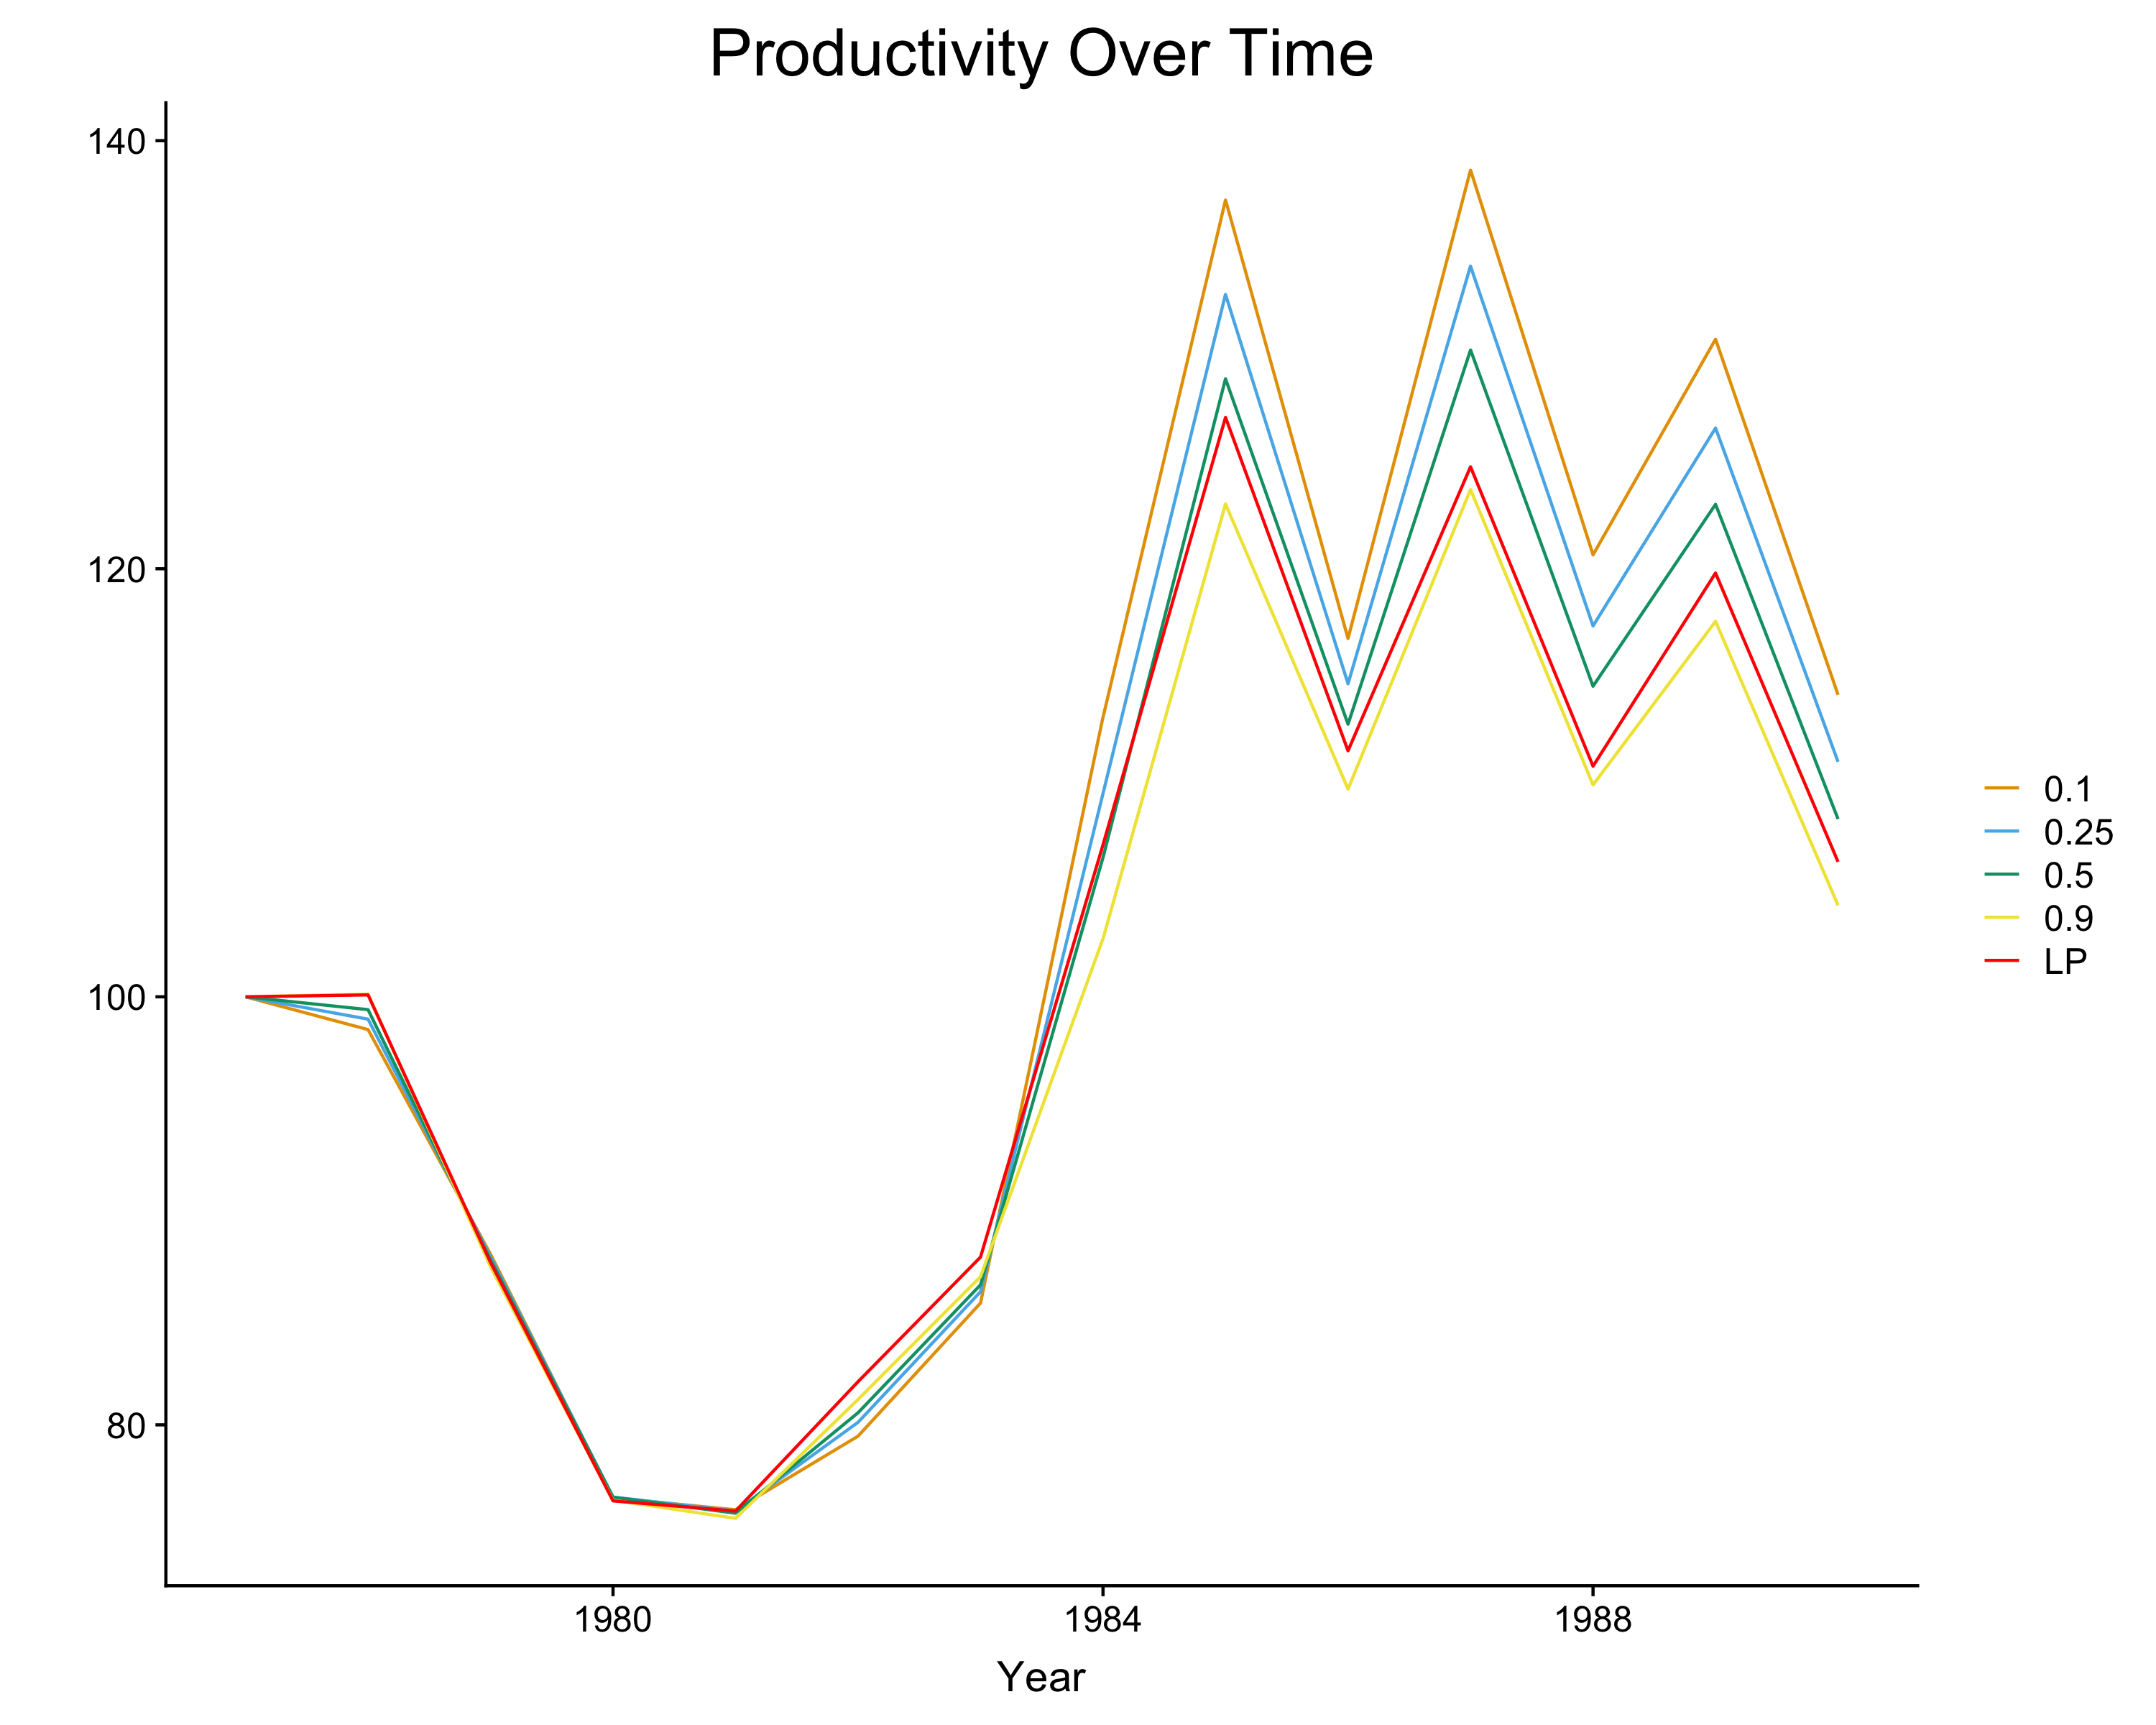
\includegraphics[width=9cm, height=7cm]{/Users/justindoty/Documents/Research/Dissertation/Production_QR_Proxy/Code/Empirical/US/Plots/TFP_Plot.png}
\caption{Estimated average TFP over time. Base productivity in 1961 is set to 100}
\end{figure}
\end{frame}
%----------------------------------------------------------------------------------
\begin{frame}
\frametitle{Conclusion}
\begin{itemize}
	\item Most estimates are consistent with prior empirical results and economic theory
		\begin{itemize}
			\item \textcite{mert}
			\item \textcite{Holmes2008}
			\item \textcite{Rajan1999}
		\end{itemize}
	\item Without controlling for productivity, estimates tend to be biased upwards
	\item Mixed results for capital estimates
	\item TFP growth growth different across the firm size distribution
	\item Still working on better bandwidth selection mechanisms
	\item Extensions to a nonlinear model using \textcite{Arellano2016}
\end{itemize}
\end{frame}

%----------------------------------------------------------------------------------------------
\begin{frame}[allowframebreaks]
\frametitle{References}
\AtNextBibliography{\small}
\printbibliography
\end{frame}

















\end{document}

